\documentclass[11pt,a4paper,ja=minimal,xelatex]{bxjsarticle}
\usepackage{zxjatype}
\usepackage{xeCJK}
\usepackage{fontspec}
\setmainfont{Times New Roman}
\setCJKmainfont{BIZ UDGothic}
\setCJKsansfont{BIZ UDGothic}
\setCJKmonofont{BIZ UDGothic}
\usepackage{amsmath,amssymb}
\usepackage{graphicx}
\usepackage{booktabs}
\usepackage{tabularx}
\usepackage{url}
\usepackage{xurl} 
\usepackage{geometry}
\geometry{left=1.5cm,right=1.5cm,top=1cm,bottom=1cm,headheight=25pt,headsep=12pt}
\usepackage{fancyhdr}
\newcommand{\HeaderLeftIndent}{15pt}   % 左からの余白（例: 0pt, 1em, 5mm）。増やすと右に寄る
\newcommand{\HeaderVerticalShift}{7pt}% 上下のずれ。正で上に、負で下に（例: 3pt で上へ, -3pt で下へ）
% -------------------------------------------------
\pagestyle{fancy}
\fancyhf{}
\fancyfoot[C]{\thepage}
\fancyheadoffset[L]{\HeaderLeftIndent}
\fancyhead[L]{\raisebox{\HeaderVerticalShift}{\parbox[t]{\dimexpr\headwidth-1em\relax}{\fontsize{10.5}{13}\selectfont プロジェクト名: 潜在空間を用いたチャット型医薬品推奨ツール\\
提案者名: 川嶋宥翔}}}
\fancypagestyle{plain}{\fancyhf{}\fancyfoot[C]{\thepage}\fancyheadoffset[L]{\HeaderLeftIndent}\fancyhead[L]{\raisebox{\HeaderVerticalShift}{\parbox[t]{\dimexpr\headwidth-1em\relax}{\fontsize{10.5}{13}\selectfont プロジェクト名: 潜在空間を用いたチャット型医薬品推奨ツール\\
提案者名: 川嶋宥翔}}}\renewcommand{\headrulewidth}{0pt}}
\renewcommand{\headrulewidth}{0pt}
\newcommand{\SectionFontSize}{12}      % セクション見出し
\newcommand{\SectionBaseline}{12}       % セクション見出しの行送り
\newcommand{\SubsectionFontSize}{10.5}  % サブセクション見出し
\newcommand{\SubsectionBaseline}{13}    % サブセクション見出しの行送り
% 本文の文字サイズは \documentclass[11pt,...] の 11pt で指定（10pt/11pt/12pt などに変更可）
\newcommand{\BodyBaselineSkip}{11pt}  % 本文の行間
\usepackage{titlesec}
\titleformat{\section}{\fontsize{\SectionFontSize}{\SectionBaseline}\selectfont\bfseries}{\thesection}{0em}{}
\titleformat{name=\section,numberless}{\fontsize{\SectionFontSize}{\SectionBaseline}\selectfont\bfseries}{}{0em}{}
\titleformat{\subsection}{\fontsize{\SubsectionFontSize}{\SubsectionBaseline}\selectfont\bfseries}{\thesubsection}{0em}{}
\titleformat{name=\subsection,numberless}{\fontsize{\SubsectionFontSize}{\SubsectionBaseline}\selectfont\bfseries}{}{0em}{}
\titlespacing*{\section}{0pt}{1em}{0.25em}
\titlespacing*{\subsection}{0pt}{0.8em}{0.2em}
\usepackage{indentfirst}
\setlength{\parindent}{1em}
\usepackage{float}
\usepackage{subcaption}
\captionsetup{font=small, justification=centering}
\captionsetup[subfigure]{font=footnotesize, justification=centering}
\usepackage{enumitem}
\usepackage{pifont}
\usepackage[draft=false,breaklinks]{hyperref}
\hypersetup{
    colorlinks=true,
    linkcolor=blue,
    citecolor=blue,
    urlcolor=blue
}

\author{}
\date{}

\begin{document}
\setlength{\baselineskip}{\BodyBaselineSkip}
\setlength{\lineskip}{0.2em}

\begin{center}
\fontsize{14}{17}\selectfont\bfseries
【提案プロジェクト詳細】
\end{center}
\begin{center}
\fontsize{10.5}{13}\selectfont
開発テーマ名：潜在空間を用いたチャット型医薬品推奨ツール\\
提案者名：川嶋宥翔
\end{center}

% ========== ① 何を作るか ==========
\section*{\ding{172} 何を作るか}

本提案は、相談内容を入力すると、ルールと潜在空間の二段構えで安全に医薬品を推奨し、根拠を表示するシステムである。

\subsection*{背景（なぜ）}
ドラッグストアで、どの薬を選べばよいか迷った経験はないだろうか。棚には似た効能の製品が並び、どれが自分に本当に合う一つを選ぶことに迷う経験は、多くの人が持っているはずだ。

私は現在、名古屋市内のドラッグストアで勤務している。耳が遠く説明を十分に聞き取れない高齢者、症状を日本語でうまく伝えられない外国人のお客様。多様な背景を持つ方々が「薬を選ぶ」という一点で困難に直面している。しかし現場は慢性的な人手不足にあり、繁忙時には一人ひとりに十分な時間を割くことができない。そのたびに、「もっと力になりたいのに」という無力感を覚えてきた。

この現場の葛藤は、個人の問題ではない。日本が直面する構造的課題と深く結びついている。

少子高齢化が進む日本では、医療機関の負担軽減が喫緊の課題である。その鍵を握るのが「セルフメディケーション」だ。これはWHOが「自らの健康に責任を持ち、軽度な不調は自分で手当てすること」と定義する概念である。実際、市場規模は拡大を続け、ドラッグストア業界は10兆円を超える産業へと成長している。しかし、その成長の裏には二つの大きな壁が存在する。「場所の壁」と「知識の壁」である。

まず「場所の壁」だ。ドラッグストアは全国に広がっているが、その分布は均一ではない。特に過疎地では「相談できる店がない」という医療アクセス格差が生じている。図\ref{fig:dragstore}は、全国の都道府県別、および和歌山県内におけるドラッグストアの分布を示したものだ（経済産業省「商業動態統計」2020年、および筆者による独自調査）。私は和歌山県有田郡有田川町という、みかんで知られる町で生まれ育った。実家の近くにドラッグストアはなく、最寄り店舗までは約5km。車がなければ薬一つ買いに行けない環境だった。地図上の空白地帯は単なるデータではなく、かつての私や家族のように、薬へのアクセスに不安を抱える人々の生活がある。

\begin{figure}[H]
  \centering
  \begin{subfigure}[t]{0.32\textwidth}
  \centering
  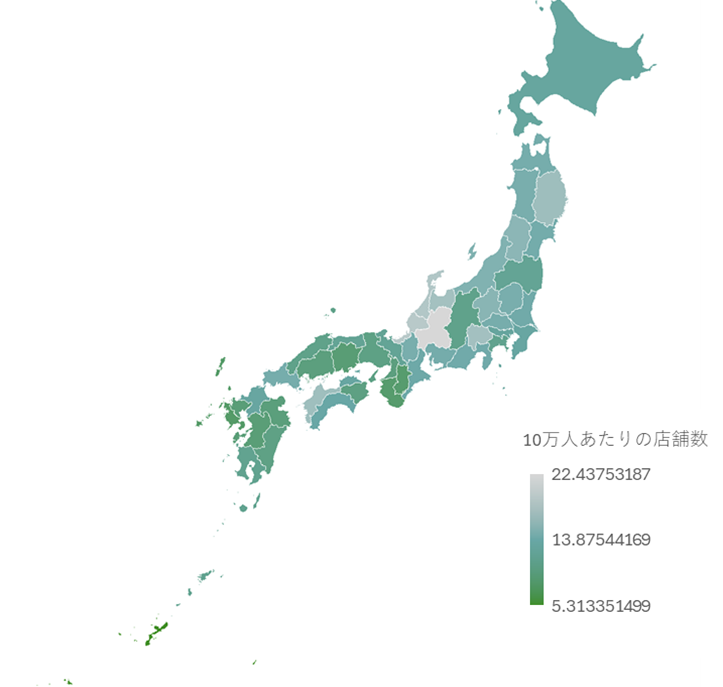
\includegraphics[width=\textwidth,keepaspectratio]{../../LaTex/photo/dragstore_injapan.png}
  \caption{都道府県別\\（経済産業省「商業動態統計」2020年）}
  \end{subfigure}
  \hfill
  \begin{subfigure}[t]{0.32\textwidth}
  \centering
  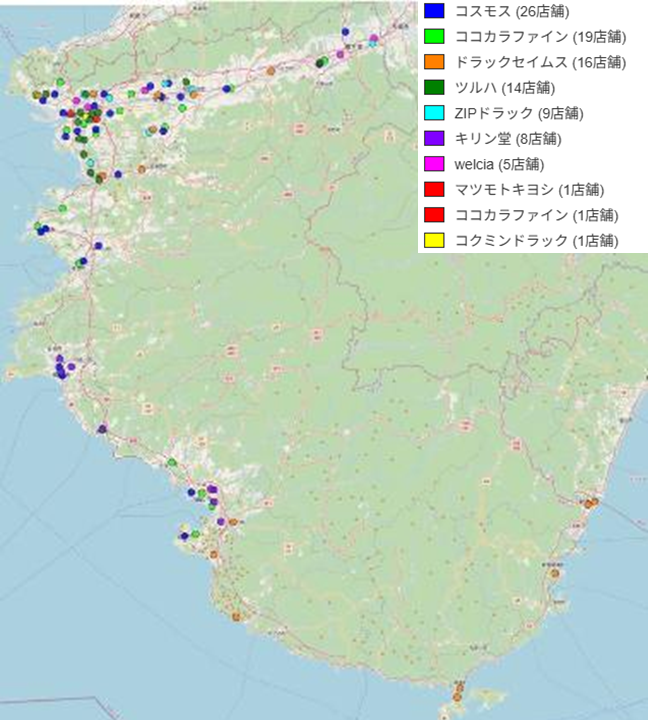
\includegraphics[width=\textwidth,keepaspectratio]{../../LaTex/photo/wakayama2.png}
  \caption{和歌山県における\\ドラッグストアの分布}
  \end{subfigure}
  \hfill
  \begin{subfigure}[t]{0.32\textwidth}
  \centering
  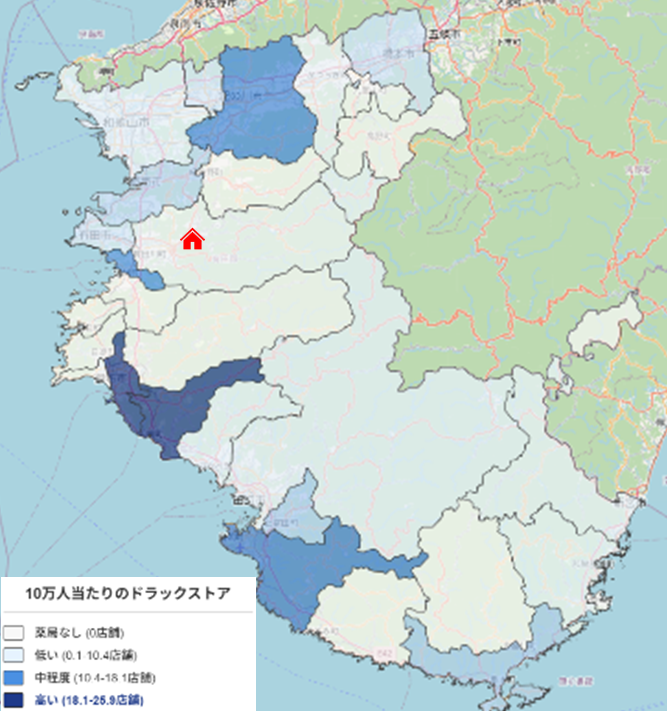
\includegraphics[width=\textwidth,keepaspectratio]{../../LaTex/photo/wakayama.png}
  \caption{人口10万人あたりの\\ドラッグストアの店舗数}
  \end{subfigure}
  \caption{ドラッグストアの地域分布}
  \label{fig:dragstore}
  \end{figure}

次に「知識の壁」である。たとえ店舗があっても、十分な専門人材が常に配置されているとは限らない。登録販売者や薬剤師の有効求人倍率は3倍を超え、慢性的な人材不足が続いている。さらに、薬機法の改正により一般用医薬品のインターネット販売が解禁され、利便性は向上した一方で、専門家の介在なしに誤った選択をしてしまうリスクも高まった。実際、市販薬の不適切使用や依存の問題は深刻化している。

つまり、日本では今、「自分で健康を守る」ことが求められているにもかかわらず、相談できる場所も、常に頼れる知識も、十分に行き渡っていないという構造的矛盾が存在している。

だからこそ私は、この「場所の壁」と「知識の壁」をテクノロジーで取り払いたい。誰もが、住む地域や言語、時間帯に関係なく、「どこでも・安心して」最適な医薬品を選択できる社会を実現する。それが本プロジェクトの出発点である。
\subsection*{目的・目標（何を・どこまで）}
本提案の\textbf{目的}は、この「選びにくさ」を解消し、\textbf{誰もが「どこでも・安心して」医薬品を選択できる}社会に貢献することである。住む場所や言語、相談環境にかかわらず適切な医薬品選択を支援し、安全なセルフメディケーションを実現できるようにする。

\vspace{0.3em}
\noindent\textbf{■ 現状のシステム（実装・本番運用済み）}

すでに以下の機能を実装し、本番環境（Neon PostgreSQL + GCP Cloud Run）で稼働している。

\begin{itemize}[nosep,leftmargin=1.5em]
  \item \textbf{ルールベース推奨エンジン}：症状を自然言語で入力すると医薬品を上位3件推奨
  \item \textbf{5層防御}（入力検証・NLU・禁忌・アレルギー・最終判定）：禁忌判定99\%以上・アレルギー98\%除外を達成（年齢・妊娠・授乳・既往症・アレルギー成分の組み合わせを網羅した独自テストケース300件による測定値。詳細は未踏期間中に安全性検証レポートとして整備する）
  \item \textbf{4言語対応}（日・英・中・韓）：訪日外国人・在留外国人にも対応
  \item \textbf{管理者インターフェース}：AIによる自動応答・手動介入・監視機能
\end{itemize}

\vspace{0.3em}
\noindent\textbf{■ 未踏期間の目標（どこまで作るか）}

現状の限界は二点ある。一点目は、ルールベースのみでは\textbf{症状表現の揺れや多様な言い回し}に対応しきれない推薦精度上の限界。二点目は、推奨結果が\textbf{文章中心の表示}であり（図\ref{fig:medicine_recommended}）、複数の推奨医薬品を並べて比較・識別することが利用者にとって難しいというUI上の課題である。未踏期間中に\textbf{潜在空間ベクトル類似度モジュール}を新たに実装・既存システムに統合し、ルールと潜在空間のハイブリッドスコアリングにより推薦精度を向上させる。あわせて、推奨結果の表示を\textbf{カルーセル型UI}（医薬品パッケージ画像・商品名・主な効能をカード形式でスワイプ表示）へ変更し、利用者が推奨医薬品を直感的に識別できるようにする。図\ref{fig:carousel-webui}はWebアプリ版カルーセルUIの実装イメージであり、図\ref{fig:line-image}はLINE版の中期実装イメージである（いずれも③節に掲載）。Webアプリ・LINE・店頭タブレットの各プラットフォームにおいて、それぞれのUIガイドラインに沿ったカード型表示として実装する。これにより、\textbf{視覚的提示による利用者の理解促進と安心感の向上}を図る。LLMは症状抽出（NLU）のみに限定することで安全性を数学的に保証しつつ精度を高める。既存の安全性指標（禁忌判定99\%以上・アレルギー98\%除外）は維持したまま、評価可能な形で検証レポートとして完成させることを目標とする。

表\ref{tab:roadmap}に現状と未踏期間の実装内容の対比を示す。

\begin{table}[H]
\centering
\caption{現状と未踏期間の実装対比}
\label{tab:roadmap}
\small
\begin{tabularx}{\textwidth}{|l|X|X|}
\hline
\multicolumn{1}{|c|}{\textbf{項目}} & \multicolumn{1}{c|}{\textbf{現状（実装済み）}} & \multicolumn{1}{c|}{\textbf{未踏期間で実装}} \\
\hline
推奨エンジン & ルールベース（禁忌・アレルギー除外） & 潜在空間ベクトル類似度を統合したハイブリッドスコアリング \\
\hline
安全性指標 & 禁忌判定99\%以上・アレルギー98\%除外 & 安全性指標を維持したまま統合・安全性検証レポート作成 \\
\hline
言語対応 & 4言語（日・英・中・韓） & 維持 \\
\hline
インフラ & Neon + GCP Cloud Run 本番稼働中 & 維持 \\
\hline
推薦精度 & ルールベースのみ（表記揺れに一部限界） & 潜在空間統合により精度向上・評価レポート化 \\
\hline
表示UI & 文章中心の推奨（候補の比較・識別が難しい） & カルーセル型UI（医薬品画像表示）、視覚的な比較を可能にする \\
\hline
管理機能 & AIによる自動応答・手動介入・監視 & 維持 \\
\hline
\end{tabularx}
\end{table}

開発の到達目標は、Phase1〜3を通じて潜在空間統合・5層防御との結合・安全性検証および評価レポートのとりまとめを完了することである（詳細な線表は④に示す）。このシステムにより、過疎地や離島でも安心して医薬品を選べる状態を目指し、住む場所による健康格差の縮小に寄与する。

\subsection*{システムの概要}
本提案で作るのは、自然言語で症状を入力すると、禁忌・アレルギーを除外したうえで、症状に合った医薬品を上位3件まで推奨するシステムである。既存のルールベース推奨エンジンを土台に、潜在空間ベクトル類似度を統合したハイブリッドスコアリングにより、推薦精度の向上を目指す。LLMは症状抽出（NLU）に限定し、推奨判断はルールと潜在空間のハイブリッドで行うため、安全性を数学的に保証できる。

\noindent\textbf{【潜在空間とは】}　潜在空間とは、単語や文章を数値ベクトルに変換した多次元の意味空間である。「頭が痛い」「頭痛がする」のように表記が異なっても、意味的に近い表現は空間上で近い位置に配置される性質を持つ。本システムでは、ユーザーの症状記述と医薬品それぞれを同じ潜在空間上に変換し、その距離（コサイン類似度）を用いて「どの医薬品が症状に最も意味的に近いか」を定量的に評価する。これにより、ルールベースでは対応しきれない症状表現の揺れや多様な言い回しにも対応できる。医薬品はPMDA（独立行政法人医薬品医療機器総合機構）が公開する添付文書情報をもとに独自に構築したもので、約8,000品目を収録している。

図\ref{fig:flowchart}に本アプリケーションの処理フロー全体を示す。医薬品推奨に至る経路では\textbf{5層防御}（入力検証・NLU・禁忌・アレルギー・最終判定）を採用し、各層の通過条件を満たした場合にのみ推奨結果を返す。安全性の主張は以下に述べる処理内容と判定条件で担保する。

\begin{figure}[H]
\centering

\includegraphics[width=\textwidth,keepaspectratio]{flowchart.png}
\caption{医薬品相談AIシステム - 処理フロー全体}
\label{fig:flowchart}
\end{figure}

本システムは、入力から推奨まで図\ref{fig:flowchart}に示す複数段階のパイプラインで処理し、各段階で安全性を確認しつつ適切に分岐する。図中の(3)〜(9)はそれぞれ5層防御のLayer1〜5に対応する。

\begin{itemize}[nosep,leftmargin=1em]
\item \textbf{(1) 属性抽出・セッション管理}（図\ref{fig:flowchart}）：ユーザー入力を受け、属性抽出を行う。セッション情報はセッション管理に渡されチャット履歴とともに保持される。
\item \textbf{(2) 入力分類（トリアージ）}：LLMにより入力をEmergency／Emotional／Physical／Ask／Otherに分類する。\textbf{Emergency}の場合は緊急応答生成から医師相談推奨・救急案内（119番等）へ分岐し処理を停止する。診断名が含まれる場合も医師相談推奨を返し薬推奨には進まない。\textbf{Ask／Other}（医薬品質問・成分・用法・店舗案内等）の場合は質問応答処理または店舗案内応答へ。\textbf{Emotional}（眠気・不眠・心の不調等）の場合はカウンセリング応答へ。\textbf{Physical}の場合のみ医薬品推奨パス（以下(3)以降）に進む。
\item \textbf{(3) セキュリティ検証}（Layer1）：ユーザー入力を解析し、プロンプトインジェクションや不適切な要求を検出するセキュリティリスクスコア$R(x)$（0--100）を算出する。判定条件は$R(x) < 80$であり、80以上の場合は推奨処理を即停止し不正利用を防止する。
\item \textbf{(4) 緊急・店舗案内等の分岐}：心臓緊急チェックで緊急と判定された場合は緊急対応フローへ。店舗案内・遺失物の質問が検出された場合は店舗案内応答へ。不適切な要求や不明な入力の場合はカウンセリングフローを開始し、対話で症状やニーズを聞き取る。店舗導入時には店内の緊急事案（不審者・傷病人・暴力等）検出にも対応可能である。
\item \textbf{(5) カウンセリング／相談への分岐}：トリアージ結果がEmotionalの場合はカウンセリングフローへ。Askの場合は医薬品質問フローへ。カウンセリングモード中は話題転換を検知し、身体症状に切り替わった場合は薬推奨フローへ接続する。
\item \textbf{(6) NLU（症状抽出）}（Layer2）：Physicalで薬推奨に進む場合、ハイブリッドNLU（辞書＋信頼度関数、閾値未満でLLMフォールバック）により入力から症状集合$S(x)$へ変換する。判定条件は$|S(x)| > 0$（最低1つ症状が抽出されること）。信用度が低い場合は質問応答処理へフォールバックする。症状分析は症状DBとOpenAI APIを利用する。
\item \textbf{(7) 禁忌チェック}（Layer3）：年齢・妊娠・授乳・既往症等を確認し、ユーザー$u$に対して禁忌$E(u)$が存在しないこと（$\lnot E(u)$）が条件。該当する場合は医師受診を促し推奨を出さない。既往症（胃潰瘍・腎疾患・喘息等）を有する場合は該当成分を含む医薬品を除外し、必要に応じて専門家への案内を優先する。
\item \textbf{(8) 医薬品候補の取得・アレルギー除外}（Layer4）：医薬品DBから候補を取得し、アレルギー成分を含む医薬品は完全除外する。推奨候補$m$とユーザー$u$について$\mathrm{allergy\_check}(m,u) = \mathrm{False}$であることが通過条件である。
\item \textbf{(9) スコアリング・最終判定}（Layer5）：ルールベーススコアと潜在空間のコサイン類似度を統合したハイブリッドスコアでランキングし、上位$k$件（$k=3$）を推奨する。効能データを参照し、応答生成で最終応答を組み立てる。
\end{itemize}

禁忌該当時は医師受診案内、緊急時は救急案内、店舗案内は案内応答、医薬品質問は医薬品質問フロー、心の不調や不明な入力はカウンセリングフローへ分岐するなど、OTCの範囲を超えるケースでは推奨を止め適切な案内を行う。以上が5層防御（入力検証・NLU・禁忌・アレルギー・最終判定）であり、すべての層を通過した場合にのみ推奨結果がユーザーに返る。不足情報がある場合は不足情報チェックを経て応答生成に渡される。画面上では、推奨結果をアドバイス・症状分析・推奨医薬品（成分重複の注意表示や年齢制限・効能を含む）として提示し、\textbf{薬剤師要請ボタン}を常時表示しており、利用者がいつでも専門家への相談に切り替えられるようにしている。図\ref{fig:medicine_recommended}に推奨結果の表示例を示す。既存システムは多言語（4言語）対応、本番はNeon（PostgreSQL）およびGCP Cloud Runで運用中であり、管理者インターフェースからAI制御・手動返信による監視・介入も可能である。4言語対応により、訪日外国人や多言語環境でのセルフメディケーション支援にも貢献できる。

\begin{figure}[H]
\centering
\begin{minipage}[t]{0.38\textwidth}
  \centering
  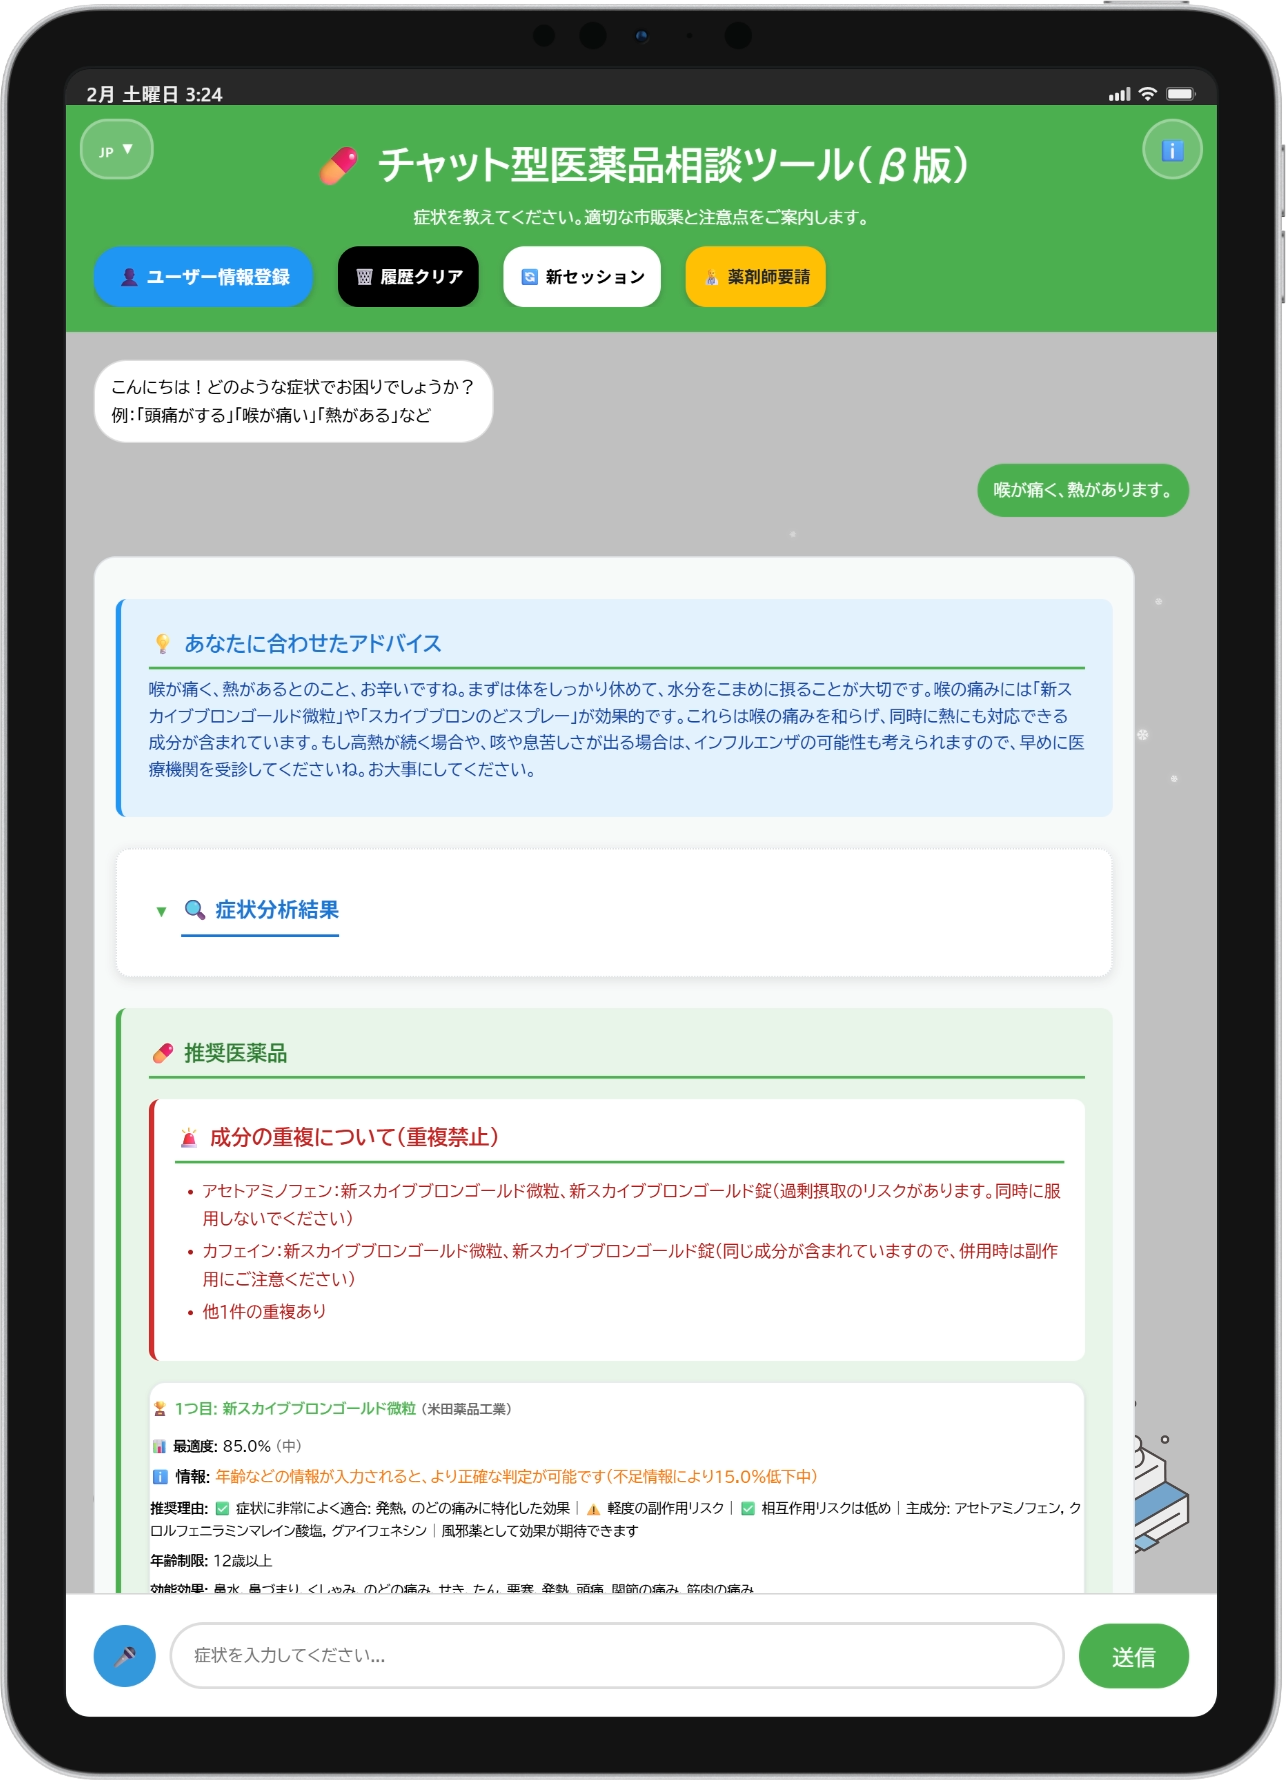
\includegraphics[width=\textwidth,keepaspectratio]{image/medicine_recomended.png}
\end{minipage}
\hfill
\begin{minipage}[t]{0.58\textwidth}
  \centering
  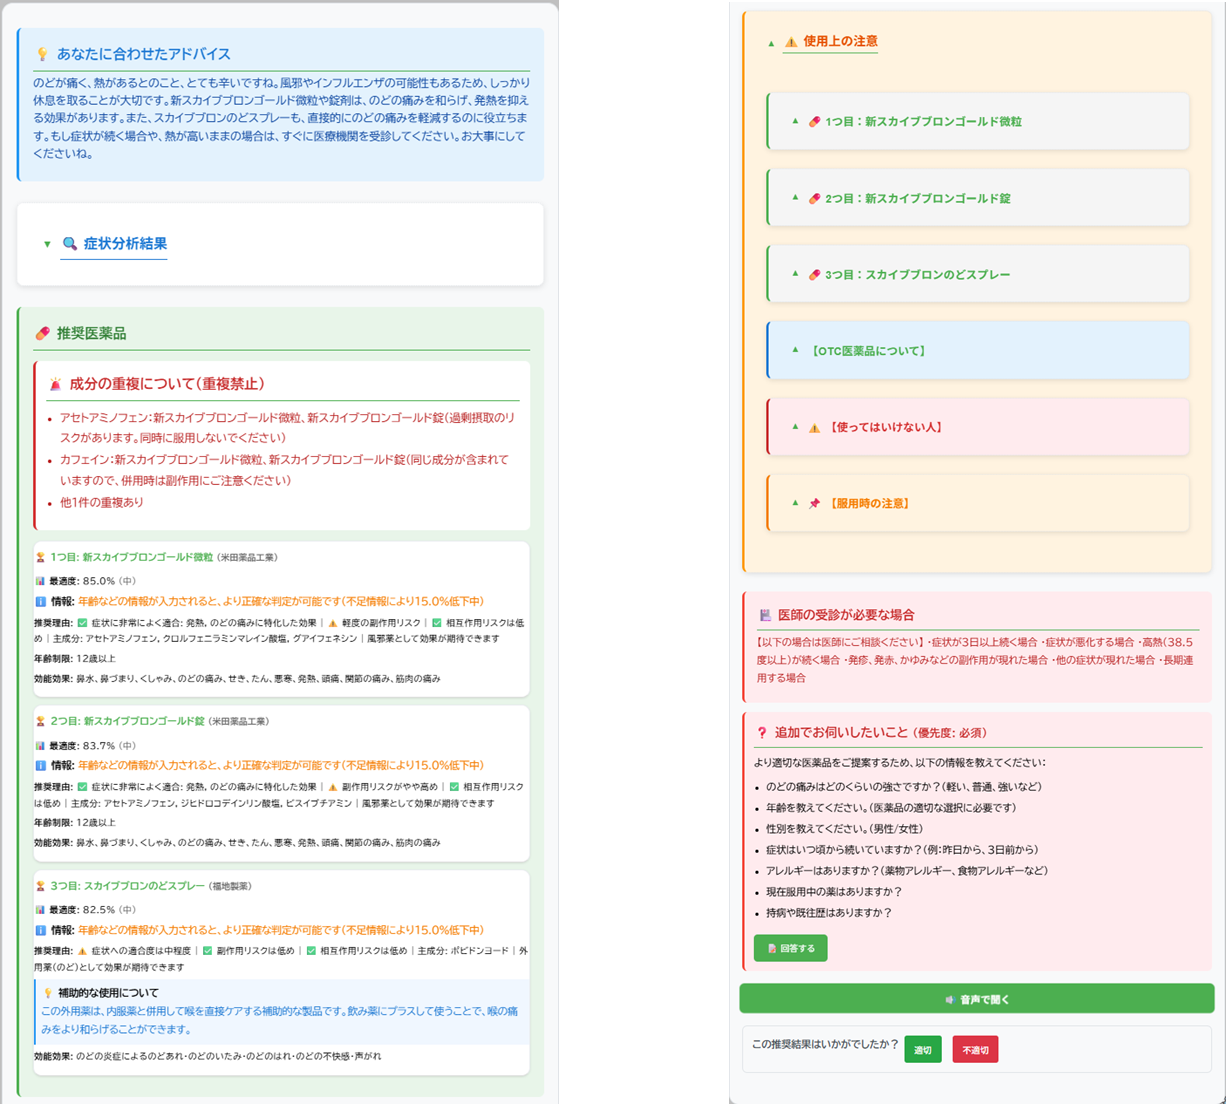
\includegraphics[width=\textwidth,keepaspectratio]{image/recommend.png}
\end{minipage}
\caption{推奨結果の表示例（左：アドバイス・症状分析・推奨医薬品・成分重複注意、右：推奨結果の全文）}
\label{fig:medicine_recommended}
\end{figure}

\begin{figure}[H]
\centering
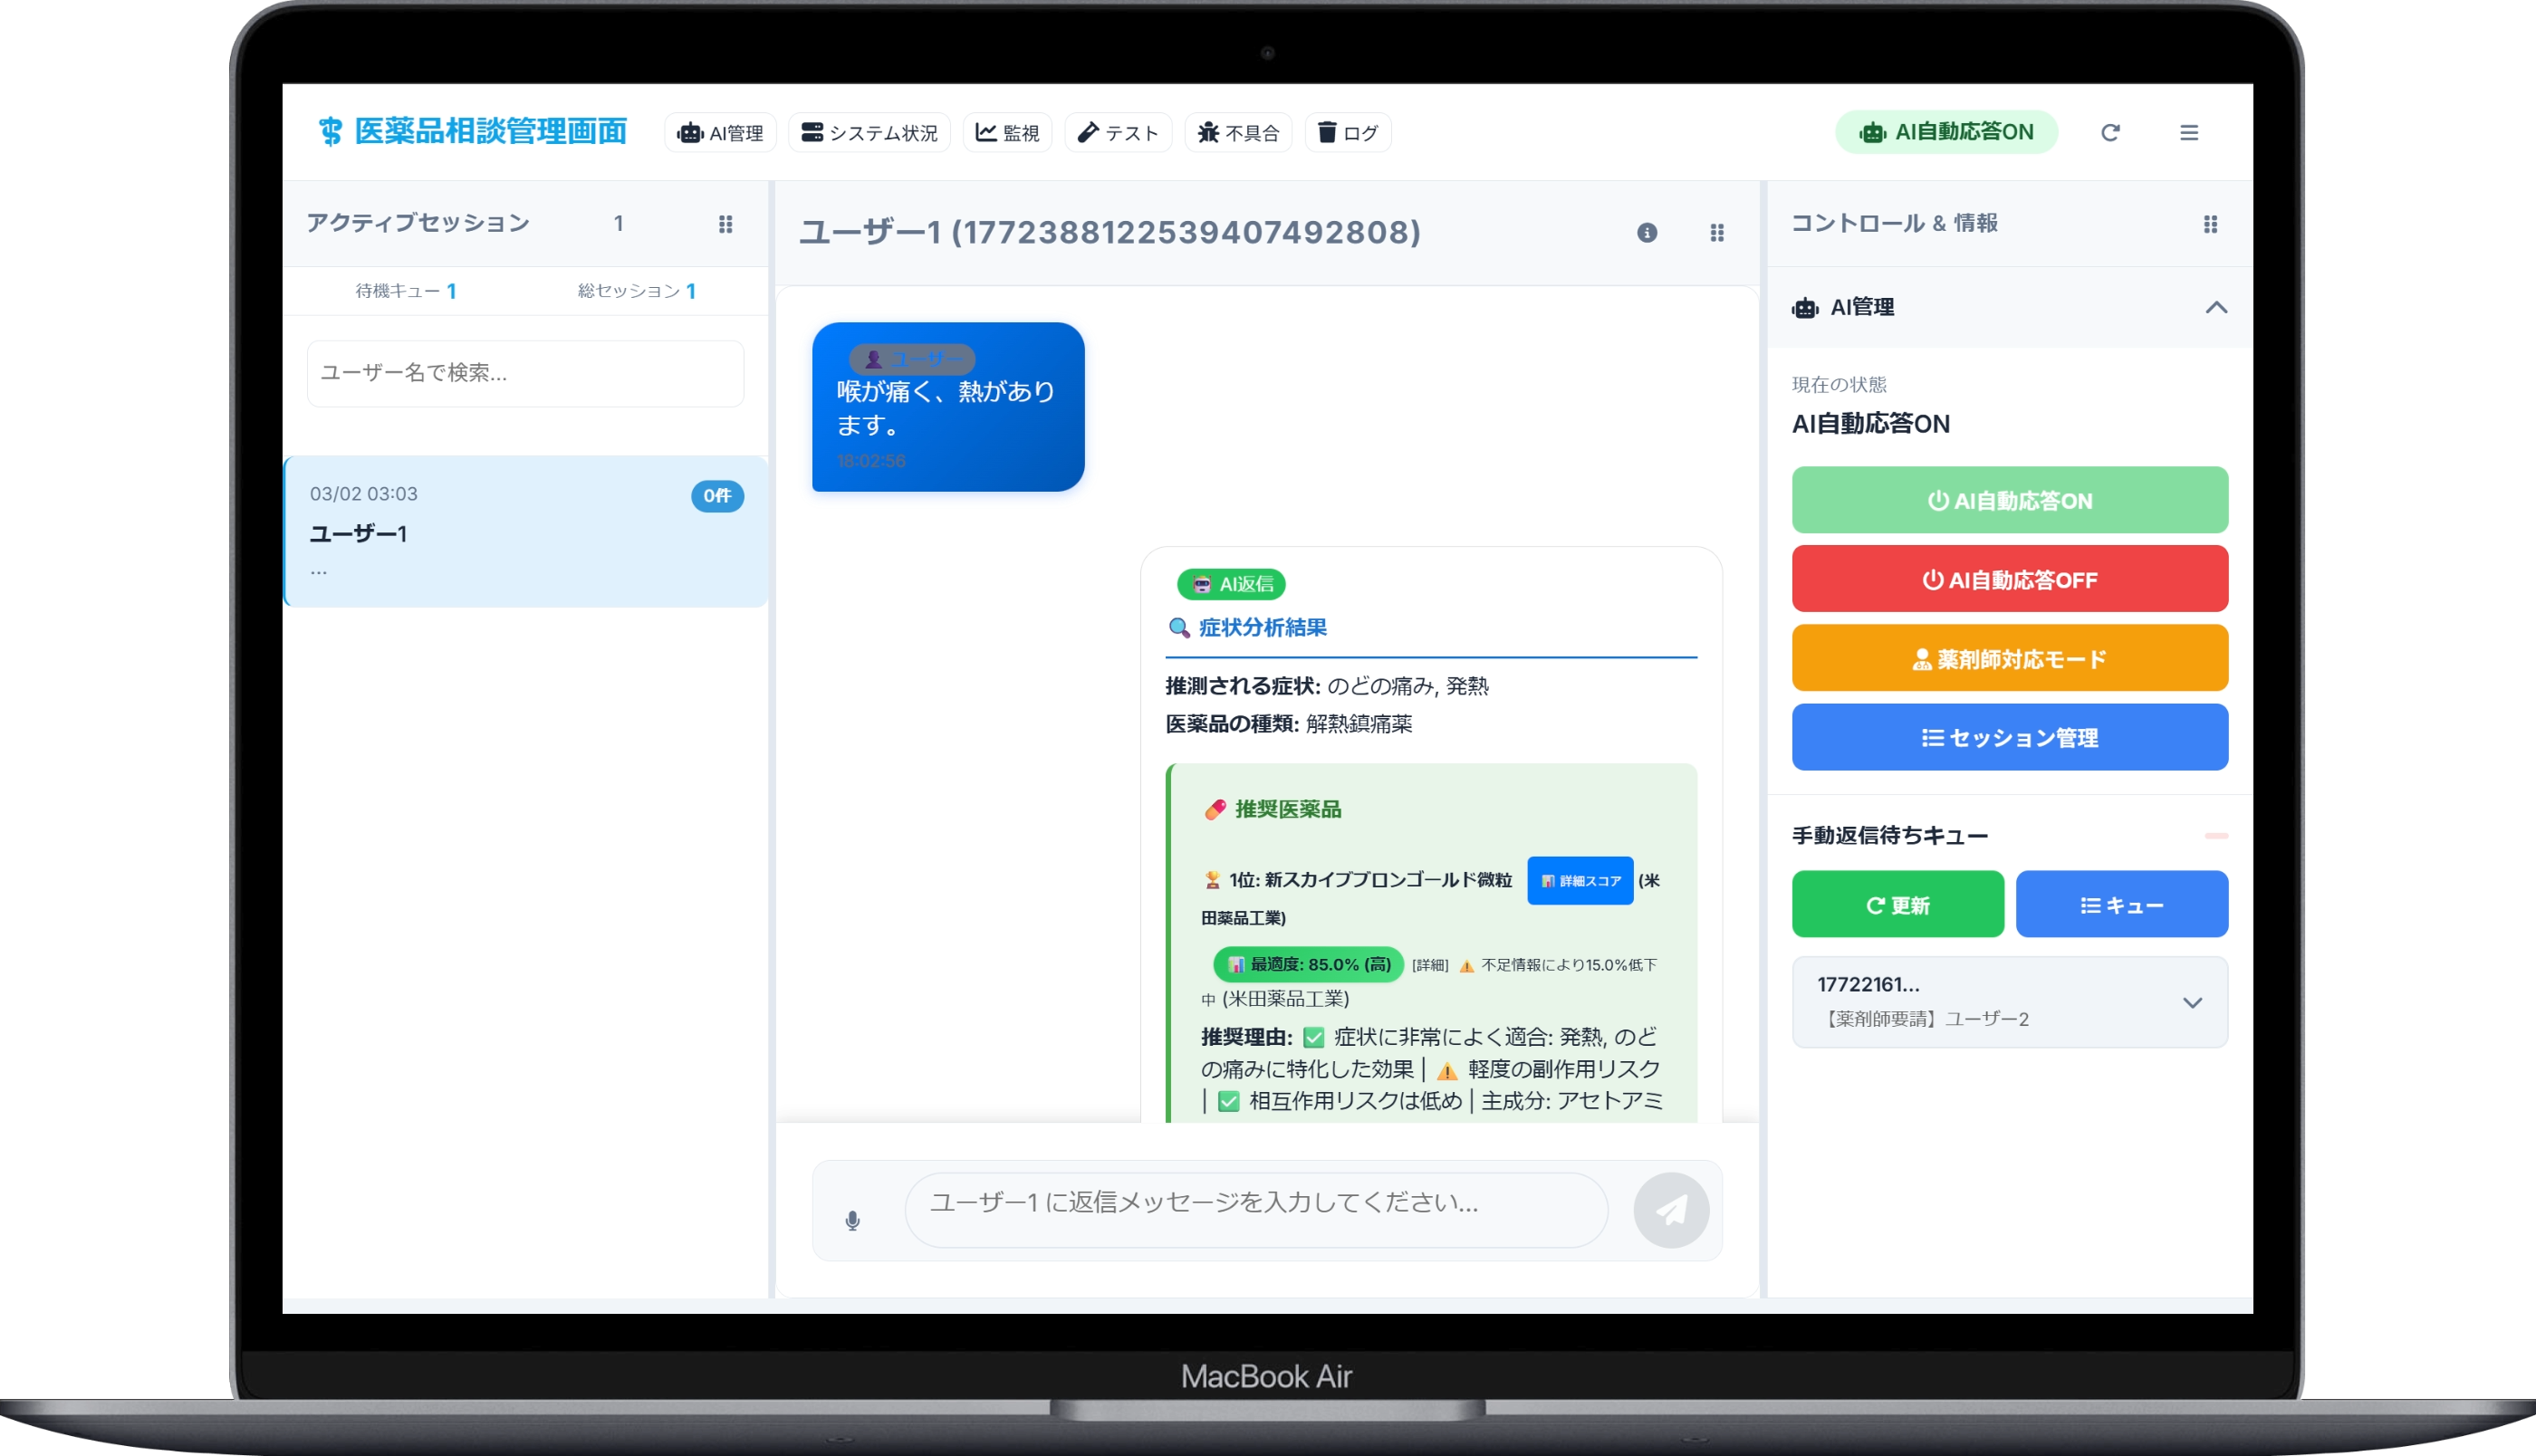
\includegraphics[width=0.8\textwidth,keepaspectratio]{image/admin.png}
\caption{管理者画面（AIによる自動応答・手動返信・監視・介入機能）}
\label{fig:admin}
\end{figure}

% ========== ② どんな出し方を考えているか ==========
\section*{\ding{173} どんな出し方を考えているか}

本プロジェクトは、訪日外国人および在留外国人の増加を見据え、日本語・英語・中国語・韓国語の4言語に対応している。LINE、行政アプリ、ドラッグストア店頭のタブレット端末など、複数のアクセス経路から利用可能な設計とし、「誰もがどこでも・安心して医薬品を選択できる社会」の実現を目指す。将来的な国際展開も視野に入れ、各国のOTC制度や販売規制の違いに適応可能な構造として設計する。図\ref{fig:language}に4言語対応の画面例を示す。

\begin{figure}[H]
\centering
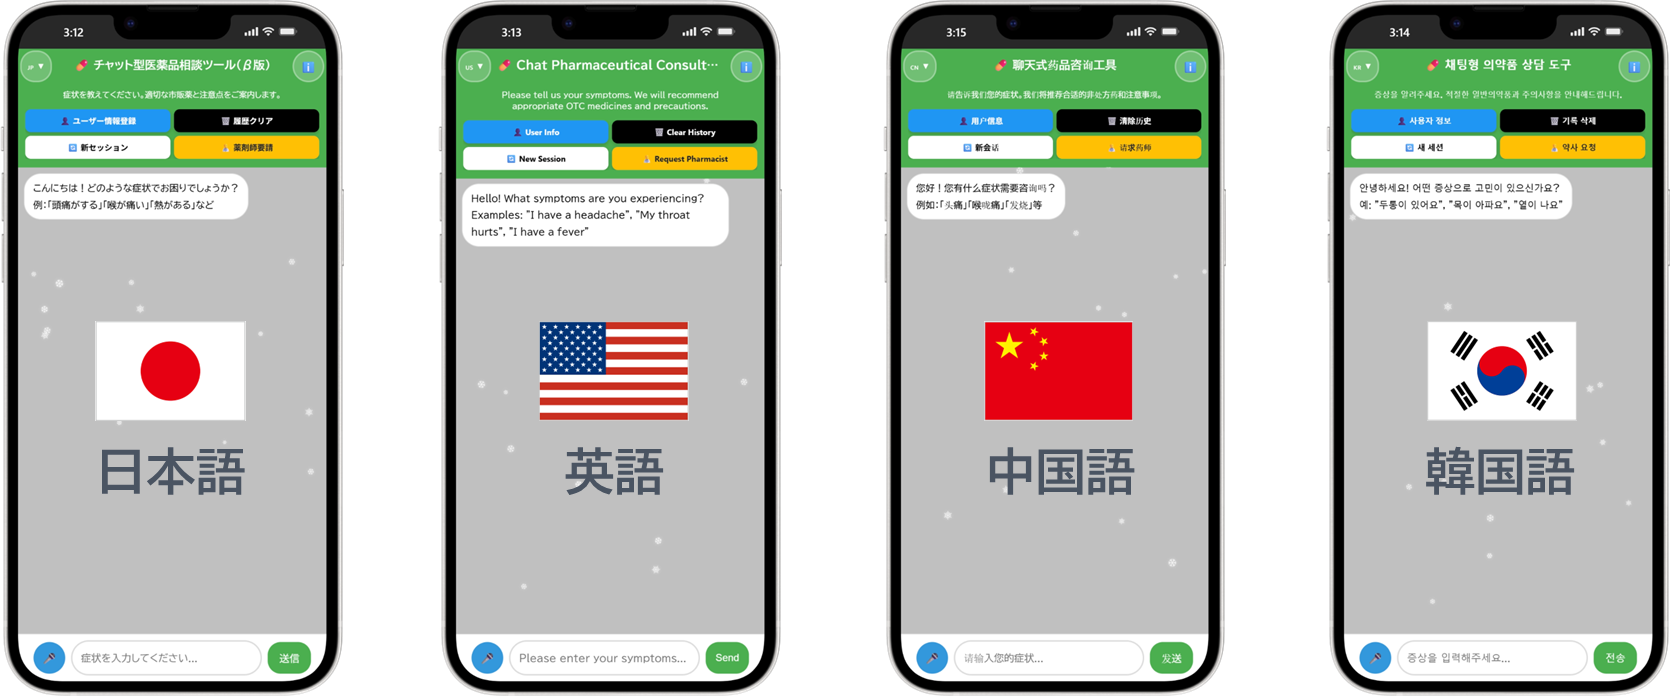
\includegraphics[width=0.85\textwidth,keepaspectratio]{image/language.png}
\caption{対応言語（日本語・英語・中国語・韓国語）の画面例}
\label{fig:language}
\end{figure}

開発したシステムの社会実装は、短期・中期・長期の三段階で進める。

\textbf{短期（未踏期間中～修了直後）}は、相談補助ツールとしてWebアプリを無料公開し、実利用環境での検証を行う。同時に、薬剤師・登録販売者による監修を並行して実施し、推奨ロジックと安全性の妥当性を専門家の視点から検証・改善する。利用者フィードバックと専門家監修の両輪で改善サイクルを回すことで、実運用に耐えうる信頼性を確立する。また、現状の文章主体の推奨表示から\textbf{カルーセル型UI}（医薬品パッケージ画像・商品名・主な効能をカード形式でスワイプ表示）への変更を実装し、未踏期間中において商品画像は代表製品を対象に手動登録による検証を進める。商品画像の視覚的提示により、利用者の理解促進と安心感の向上を図る。

\textbf{中期}には、LINE Messaging APIを活用したLINE公式アカウントを公開し（図\ref{fig:carousel-all}右）、チャット形式で気軽に相談できる環境を整備する。さらに、Yahoo!ショッピング商品検索APIを活用し、推奨医薬品のパッケージ画像をリアルタイム取得・表示するビジュアル推奨機能を実装する（アフィリエイト義務がなく楽天市場APIより制限が少ない点を踏まえ選定。利用規約に従い商品ページへのリンクを合わせて提示する）。視覚的提示により、利用者の理解促進と安心感の向上を図る。あわせて、コア技術（ルールベーススコアリング、5層防御、安全性保証設計、NLU統合部分等）のOSS化を検討し、外部検証を受ける体制を整える。情報処理学会や医療情報学関連学会での発表も視野に入れ、技術的妥当性と社会的意義の両面で評価を獲得する。

\textbf{長期（修了後）}は、実務経験を踏まえたうえで、未踏アドバンスト等の枠組みを活用し、ドラッグストア向けSaaSやAPI提供としての実用化を目指す。画像基盤については、製薬メーカーと直接交渉を行い、外装・内装・剤形を含む自前の医薬品画像データベースの構築を目指す。これによりEC系APIへの依存を脱却し、規約制約を受けない安定運用を実現する。エンドユーザー向けには無料利用を維持しつつ、店舗向けSaaS等による持続可能なビジネスモデルへと展開する。

本プロジェクトは、単なるアプリ公開にとどまらない。技術的妥当性、専門家監修、制度対応、ビジネス持続性を段階的に積み上げながら、社会基盤として定着させることを最終目標としている。

% ========== ③ 斬新さの主張・期待される効果 ==========
\section*{\ding{174} 斬新さの主張・期待される効果}

\subsection*{既存調査に基づく位置づけ}
医薬品推奨・OTC相談の手段としては、従来のドラッグストアや薬局で薬剤師・登録販売者に直接相談する方法や近年では、オンライン診療や遠隔服薬指導などの医療サービスも普及しつつある。しかし、これらの方法では高い安心感が得られる一方で、移動時間や待ち時間、予約の手間がかかり、気軽に利用しづらい場面も多い。また、最近ではGoogle検索や生成AIを用いて症状を検索・相談する方法も一般的になってきているが、推奨根拠の不透明性・禁忌やアレルギー判定の保証不可・ハルシネーションによる誤情報・医師法や薬剤師法上のグレーゾーンなど、安全性の観点で看過できない課題がある。

なお、本システムの法的位置づけについては、名古屋市健康福祉局生活衛生部環境薬務課に照会し、「診断を行わないためSaMD（Software as a Medical Device：医療機器ソフトウェア）に該当しない」との見解を得ている（正式な厚生労働省判断ではなく行政窓口への確認であることを明記する）。OTCの範囲を超えるケースでは推奨を止め医師・薬剤師への案内を行う設計としており、医師法・薬剤師法上の診断・調剤行為には一切関与しない。

こうした課題を受け、OTCに特化した医薬品相談サービスも存在するが、それぞれ限界がある。症状選択型問診のUbie、漢方特化のYOJO、従業員向けのDカウンセラーneoなどが代表例であり、固定問診・キーワードマッチ・特定領域への特化という点で対話型の汎用性を欠く。図\ref{fig:competition}はこれらと本提案システムを比較したものであり、図\ref{fig:positioning}は「安全性」と「汎用性」の二軸でのポジショニングマップである（対話型AIと5層防御・ハイブリッドスコアの両立により、高安全性かつ高汎用性の領域を狙う）。

\begin{figure}[H]
\centering
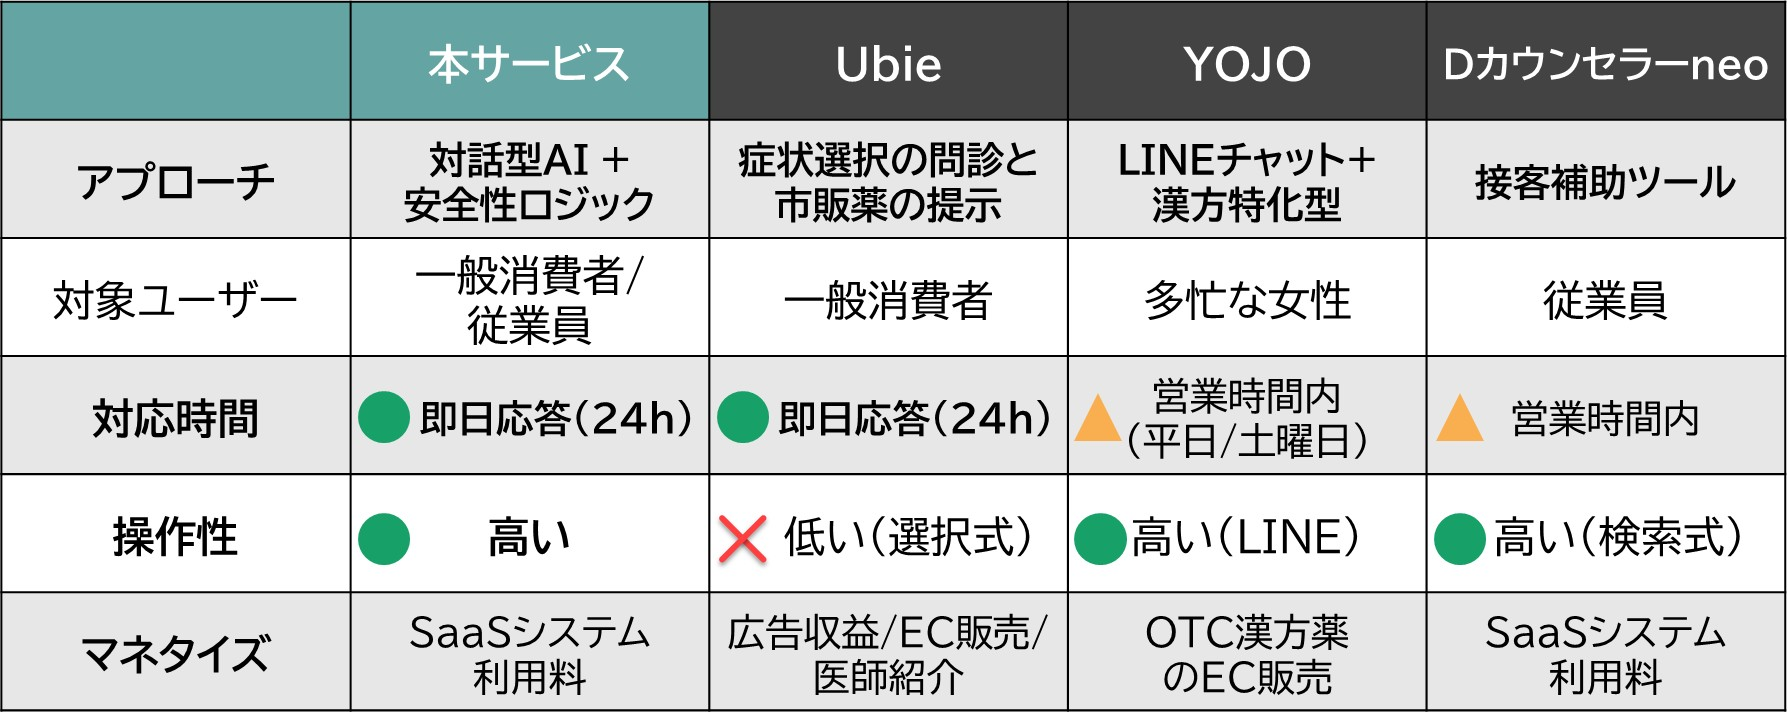
\includegraphics[width=0.6\textwidth,keepaspectratio]{image/competition.jpg}
\caption{競合との比較}
\label{fig:competition}
\end{figure}

\begin{figure}[H]
\centering
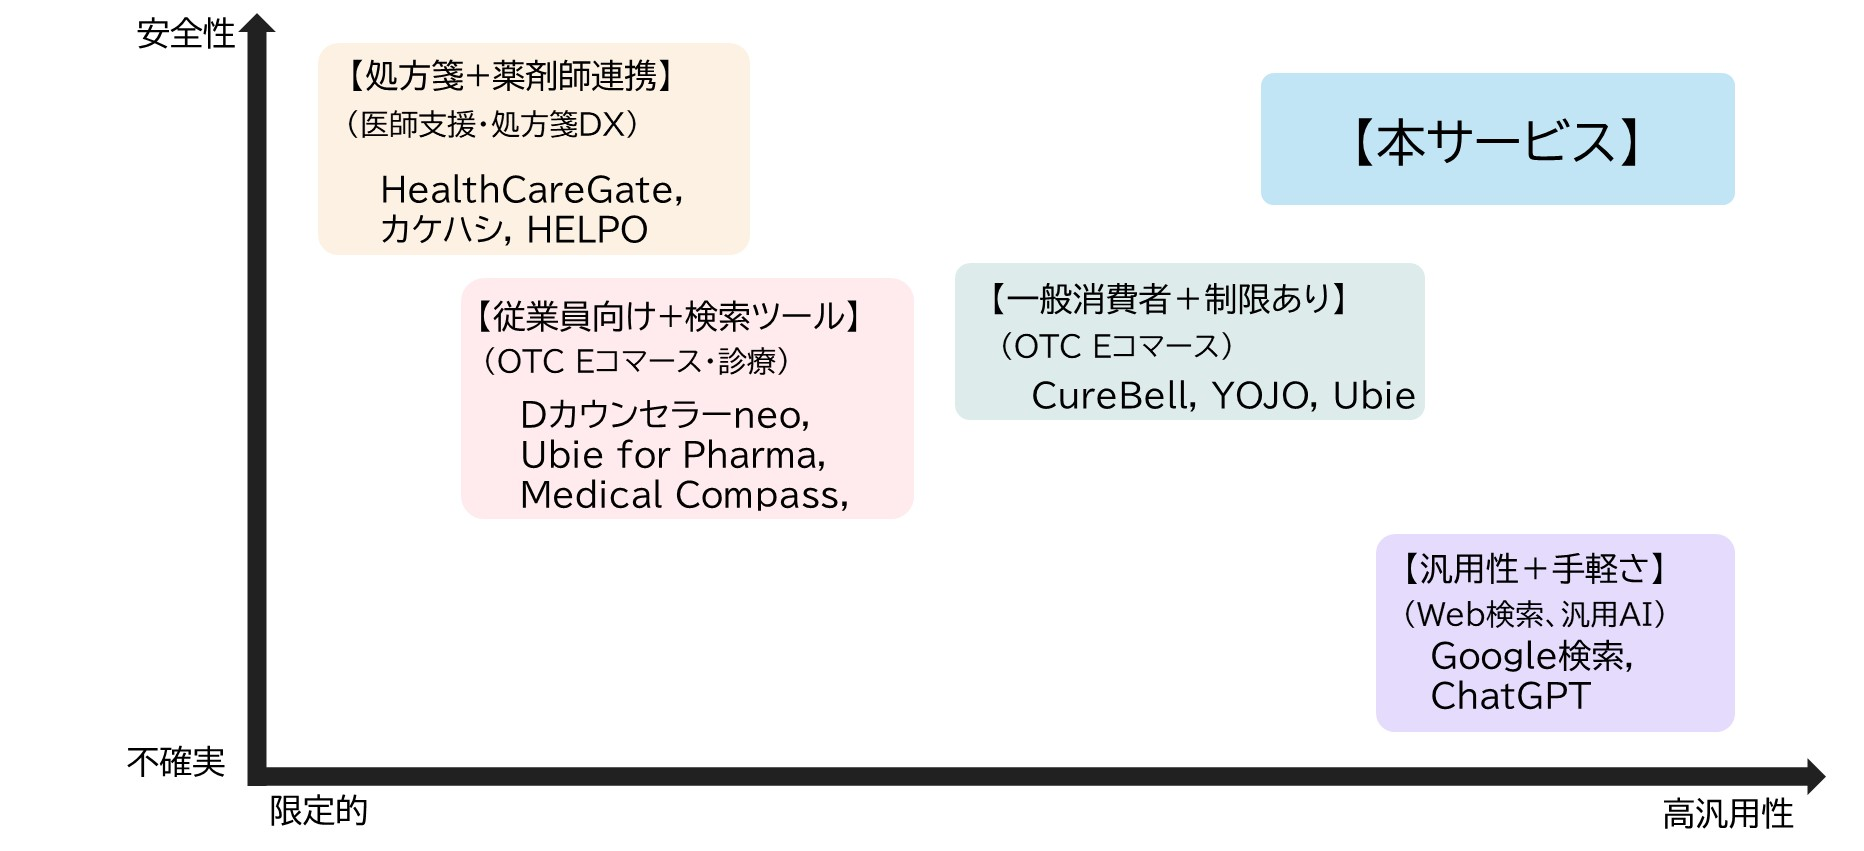
\includegraphics[width=0.6\textwidth,keepaspectratio]{image/positioning_map.jpg}
\caption{ポジショニングマップ（安全性×汎用性）。}
\label{fig:positioning}
\end{figure}

こうした既存手段・サービスの限界を技術的に整理すると、純粋な生成AIは自然言語の柔軟な理解を得意とするが、前述の通り安全性を数学的に保証できない。一方、\textbf{純ルールベース型}は透明性と安全性は高いが、症状表現の多様性に対応しづらい。既存のOTC相談ツールや薬局向けシステムの多くはキーワードマッチや固定ルールに依存しており、症状文の意味的類似度を活かした推奨が十分に実現されていない。本提案では、LLMを\textbf{NLU（症状抽出）に限定}して柔軟な理解を確保しつつ、推奨判断は\textbf{ルールベースと潜在空間ベクトル類似度のハイブリッド}で行うことで双方の欠点を克服する。潜在空間とルールベースを数理的に統合することで、安全性を保証しながら汎用的な推奨を実現する点が本提案の核心である。

技術的差別化に加え、\textbf{プラットフォーム面の差別化}も本提案の核心のひとつである。中期には、LINE Messaging APIを活用し、\textbf{日常のLINE上で完結する}カルーセル型医薬品相談サービスを公式アカウントとして展開する（図\ref{fig:carousel-all}）。LINEは国内月間アクティブユーザー約1億人（総人口の約85\%）に達し、専用アプリの追加インストールが一切不要である。既存のOTC相談ツール（Ubie・YOJO等）がいずれも専用アプリや専用サービスへの遷移を前提とするのに対し、本提案は\textbf{導入ハードルをゼロ}にする。カルーセル形式で推奨医薬品の画像・商品名・効能をスワイプで比較できるUIは、文章主体の既存ツールにはない\textbf{直感的な選択体験}を提供する。プッシュ通知による継続フォローや薬剤師への引き継ぎとも連携し、24時間・場所を問わない医薬品相談インフラとして機能させる。

\begin{figure}[H]
\centering
\begin{subfigure}[t]{0.45\textwidth}
  \centering
  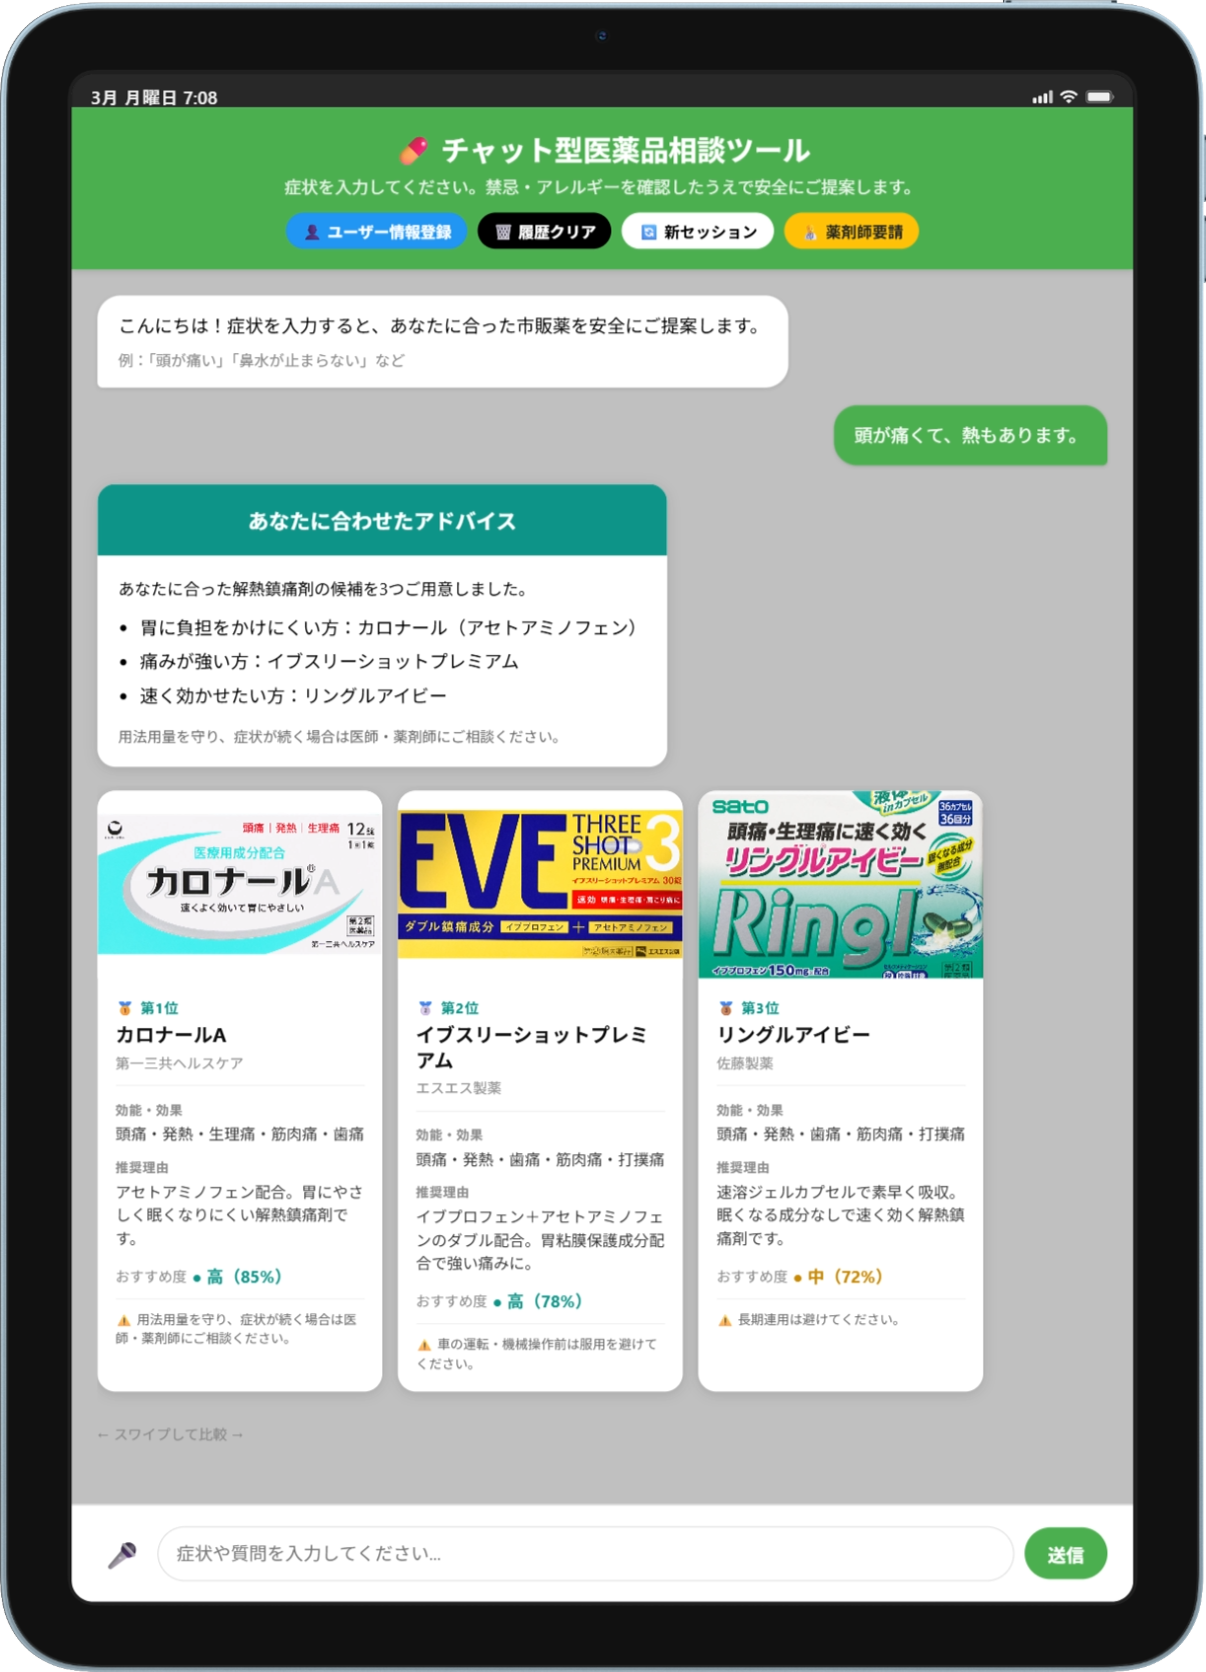
\includegraphics[width=\textwidth,keepaspectratio]{image/carousel_webui.png}
  \caption{Webアプリ版カルーセルUI（未踏期間中に実装）。症状分析・推奨理由・おすすめ度をカード形式でスワイプ比較。}
  \label{fig:carousel-webui}
\end{subfigure}
\hfill
\begin{subfigure}[t]{0.45\textwidth}
  \centering
  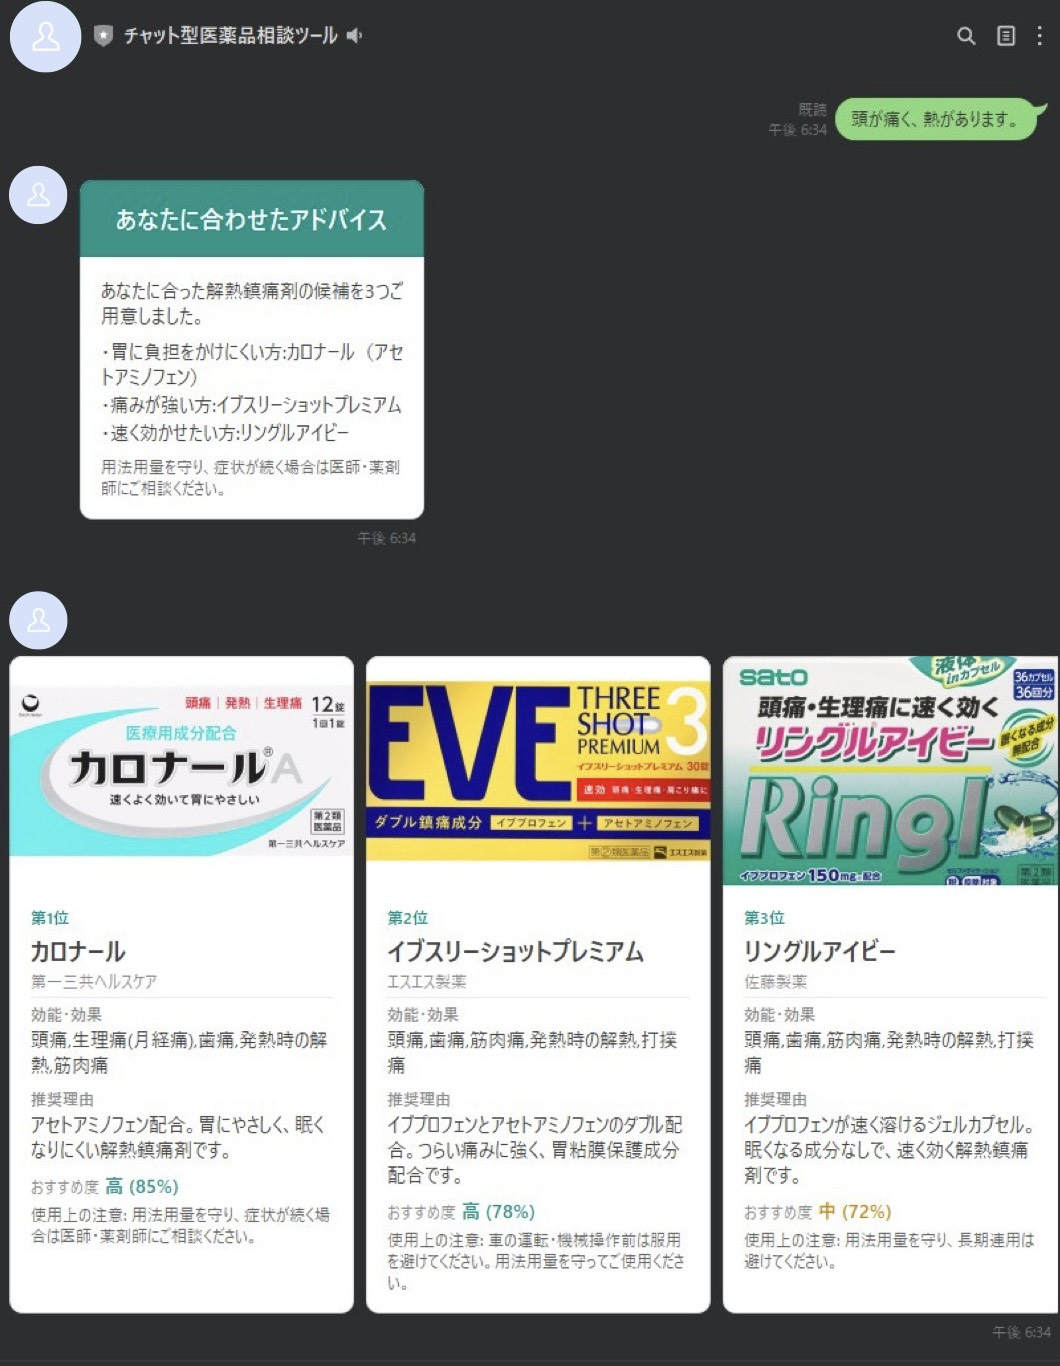
\includegraphics[width=\textwidth,keepaspectratio]{image/line_image.jpg}
  \caption{LINEカルーセル形式による医薬品推奨（中期実装予定）。}
  \label{fig:line-image}
\end{subfigure}
\caption{カルーセル型UI実装イメージ。左：Webアプリ版（未踏期間中）右：LINE版（中期）\\
いずれも医薬品パッケージ画像・商品名・効能・推奨理由をカード形式でスワイプ比較できる。}
\label{fig:carousel-all}
\end{figure}

\subsection*{技術的な裏付け}
本提案の設計思想は\textbf{「人が誤らないための構造を提供する」}ことにある。判断を機械に丸投げするのではなく、禁忌・アレルギーはルールで先に除外し、説明可能な形で推奨根拠を提示する。これにより、利用者は自身の責任の範囲を理解したうえで選択できる。

\begin{itemize}[nosep]
\item \textbf{5層防御}: 推奨が成立するためには、入力検証・NLU・禁忌・アレルギー・最終判定の各層がすべて通過する必要がある。禁忌・アレルギーはルール層で先に除外し、潜在空間の類似度は「除外後の候補」に対するスコア付けにのみ用いるため、安全性が数学的に保証される。
\item \textbf{ハイブリッドスコア}: $S(m,u) = \alpha \cdot \mathrm{sim}(v_u, v_m) + \beta \cdot \mathrm{coverage}(S_u, E_m) - \delta \cdot \mathrm{penalty}(m,u)$ により、症状と医薬品効能の意味的類似度と、既存ルール（カバレッジ・ペナルティ）を統合する。なお、$\mathrm{coverage}$（症状カバレッジ）と$\mathrm{penalty}$（禁忌・重複ペナルティ）はルールベースとして既に実装済みである。未踏期間の主要タスクは、$\mathrm{sim}(v_u, v_m)$（潜在空間ベクトルのコサイン類似度）を新たに実装し、この式に統合することである。信頼度に応じた動的重みを導入し、曖昧な入力時は潜在空間をやや重視する設計とする。
\item \textbf{アクセシビリティ設計}: 高齢者や外国人を含む多様な利用者が初めてでも迷わず使えるよう、マイクによる\textbf{音声入力}と\textbf{音声読み上げ}機能を実装している。文字入力が苦手な高齢者でも自然な発話で症状を伝えられ、応答を音声で確認できる設計である。初回起動時には言語選択・利用上の注意・操作方法を順を追って案内する直感的なオンボーディングガイドを搭載しており（図\ref{fig:onboarding}）、誤用防止という5層防御の一環としても機能する。
\end{itemize}

\begin{figure}[H]
\centering
\begin{center}
\begin{subfigure}[t]{0.17\textwidth}
  \centering
  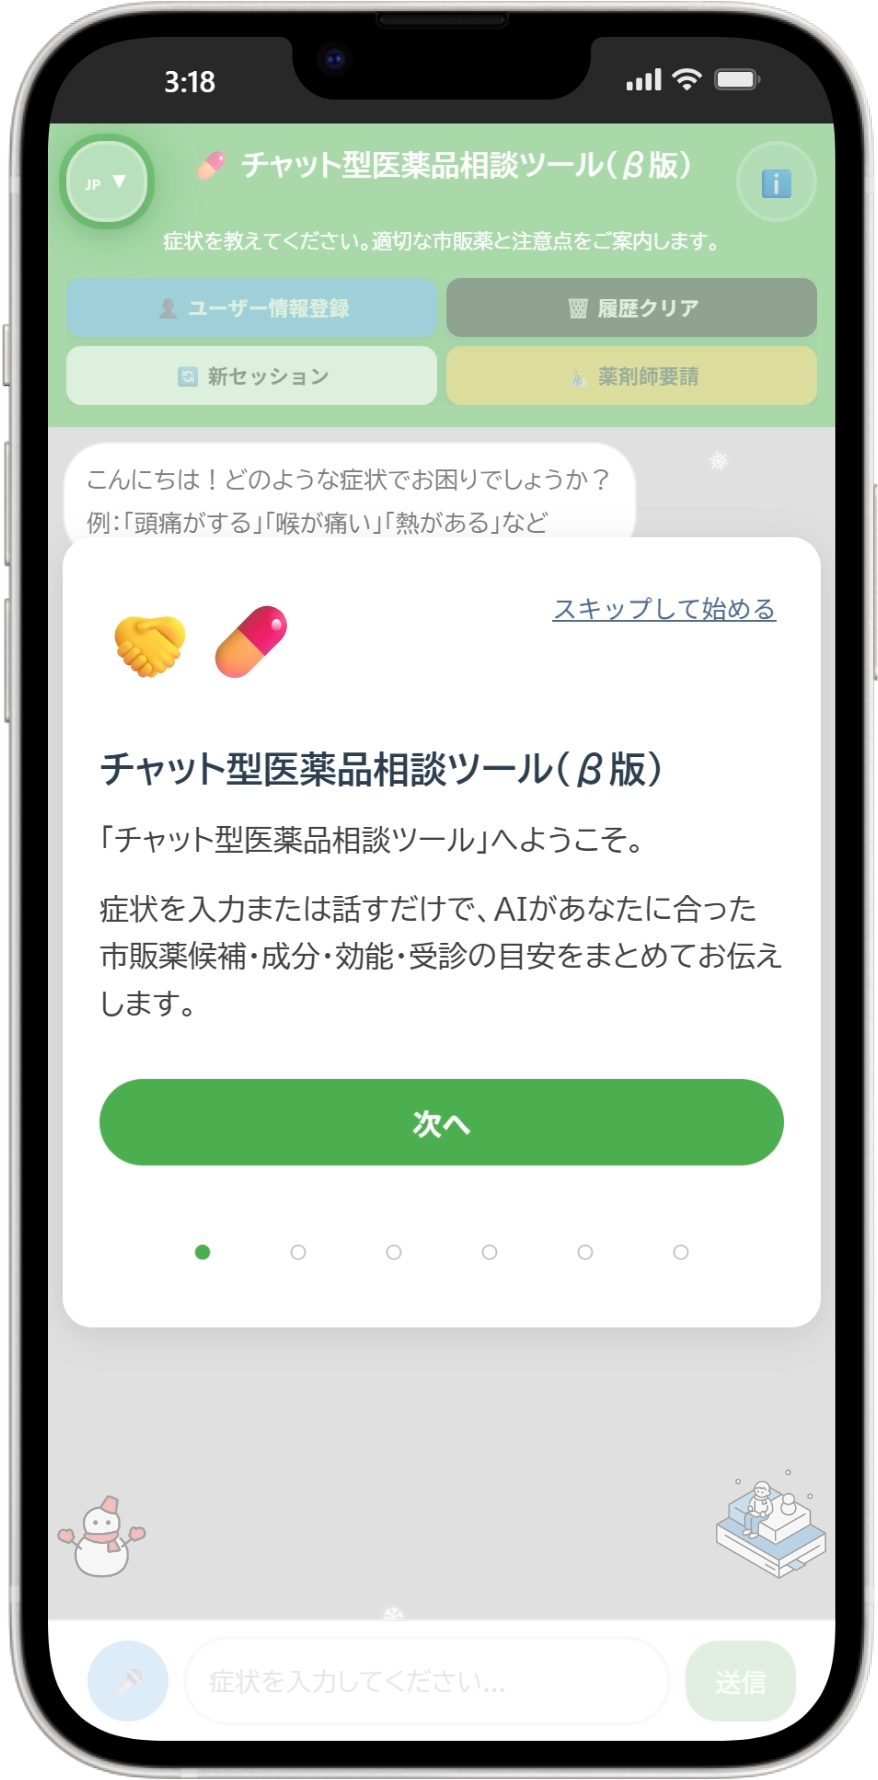
\includegraphics[width=\textwidth,keepaspectratio]{image/onboarding1.png}
\end{subfigure}
\begin{subfigure}[t]{0.17\textwidth}
  \centering
  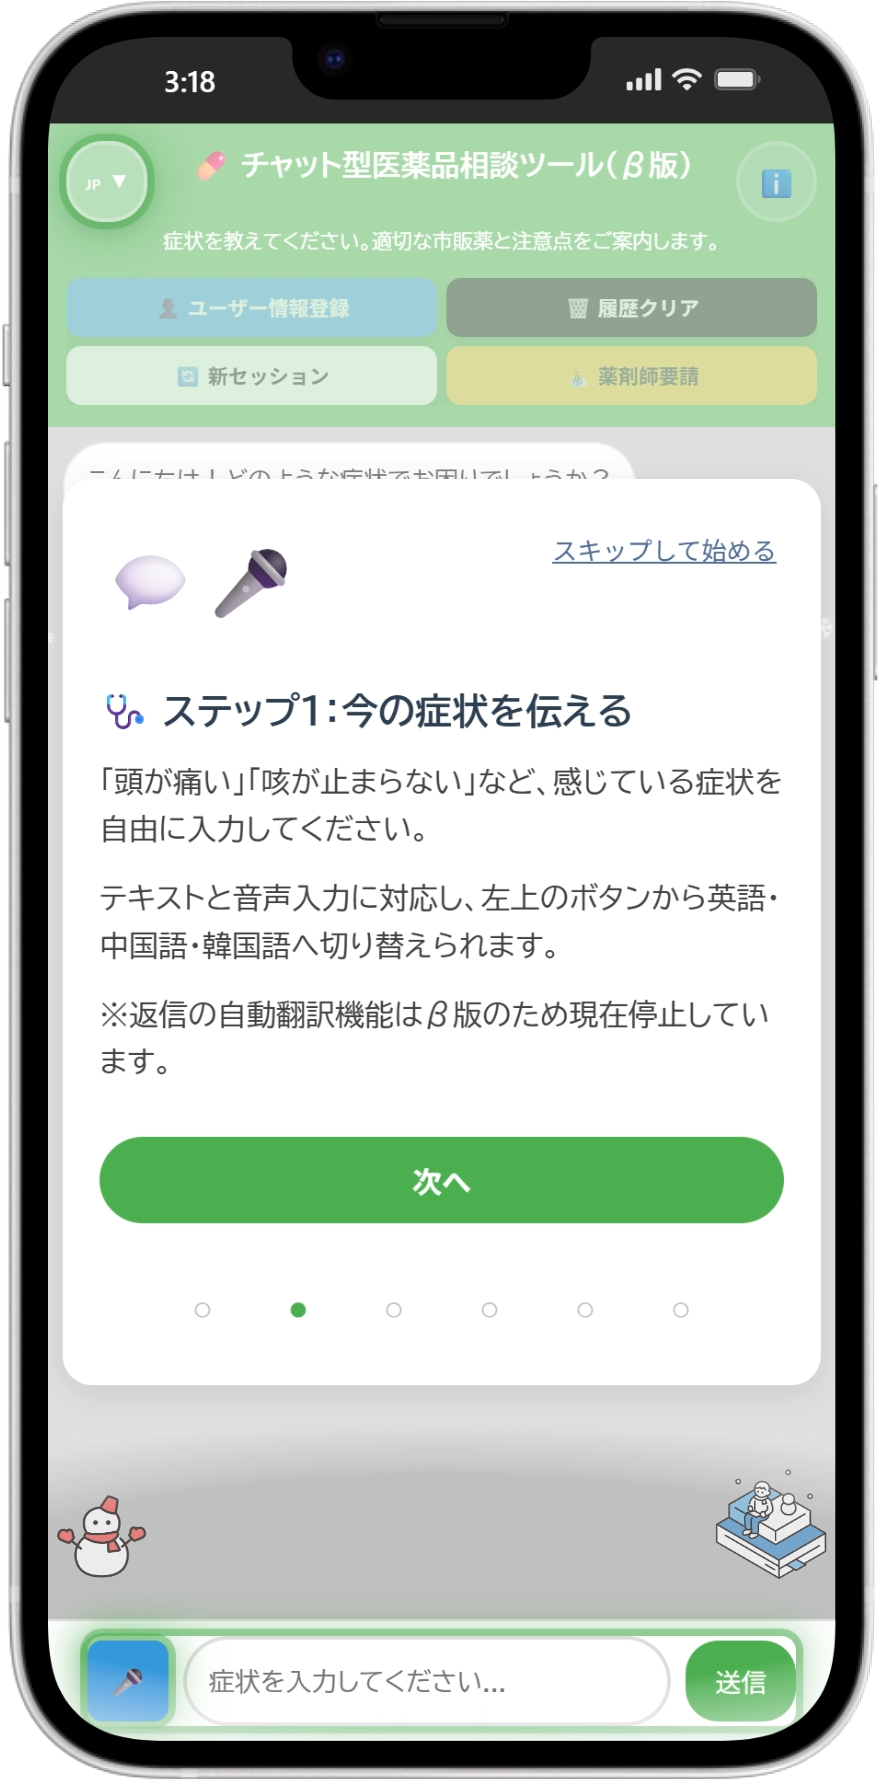
\includegraphics[width=\textwidth,keepaspectratio]{image/onboarding2.png}
\end{subfigure}
\begin{subfigure}[t]{0.17\textwidth}
  \centering
  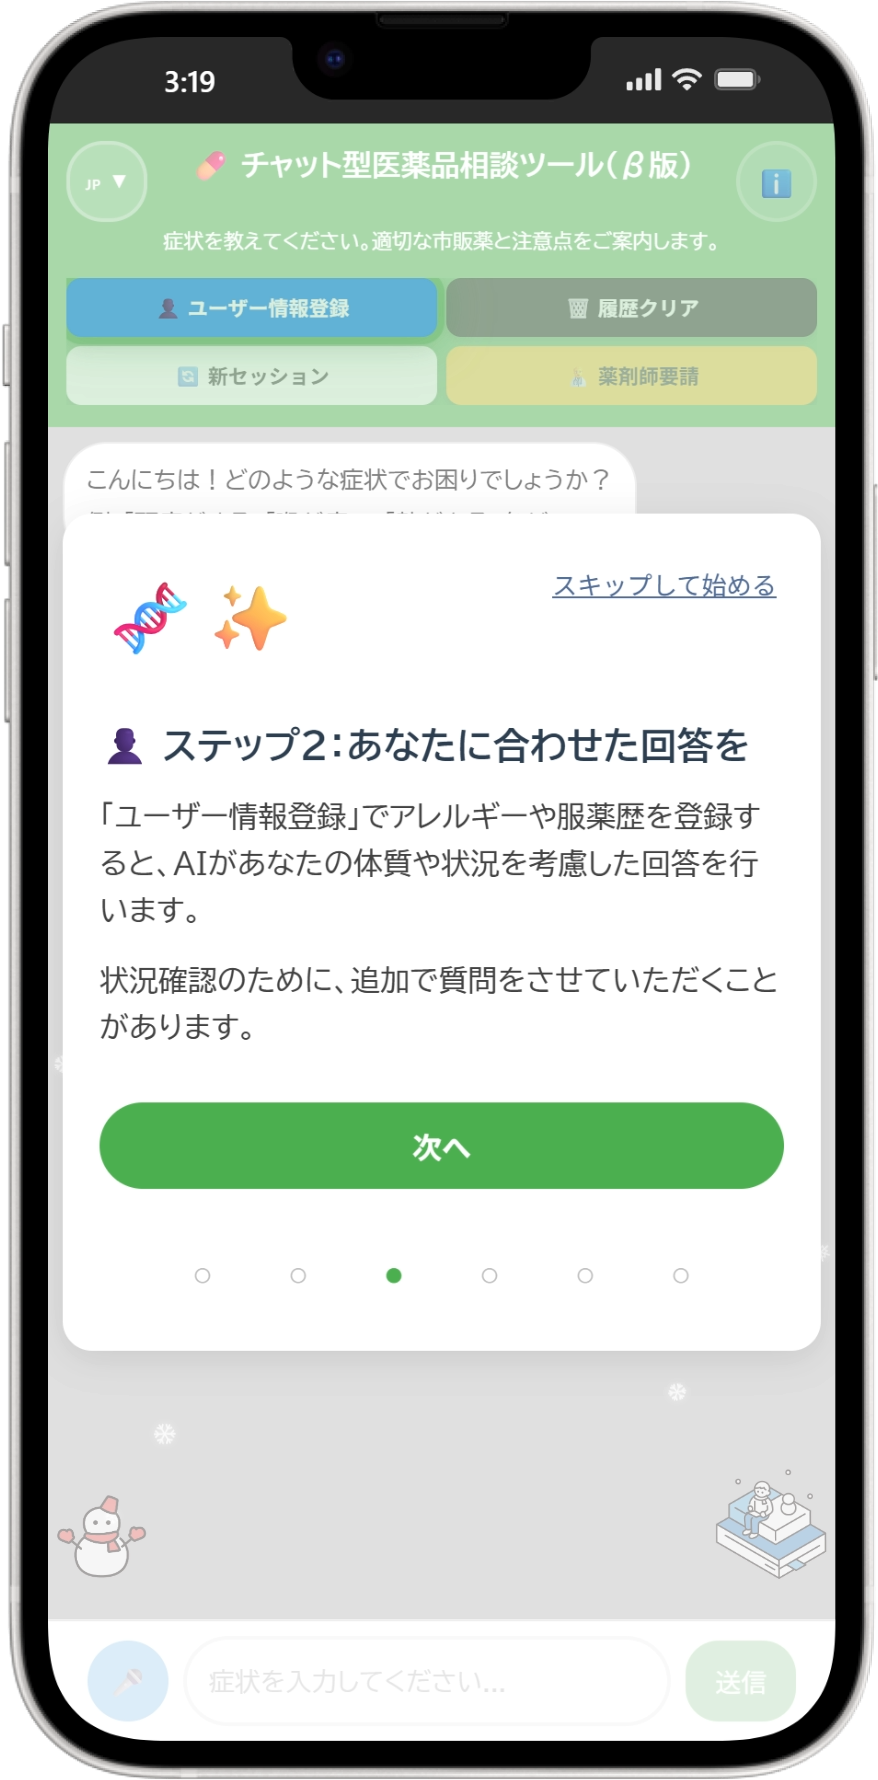
\includegraphics[width=\textwidth,keepaspectratio]{image/onboarding3.png}
\end{subfigure}
\begin{subfigure}[t]{0.17\textwidth}
  \centering
  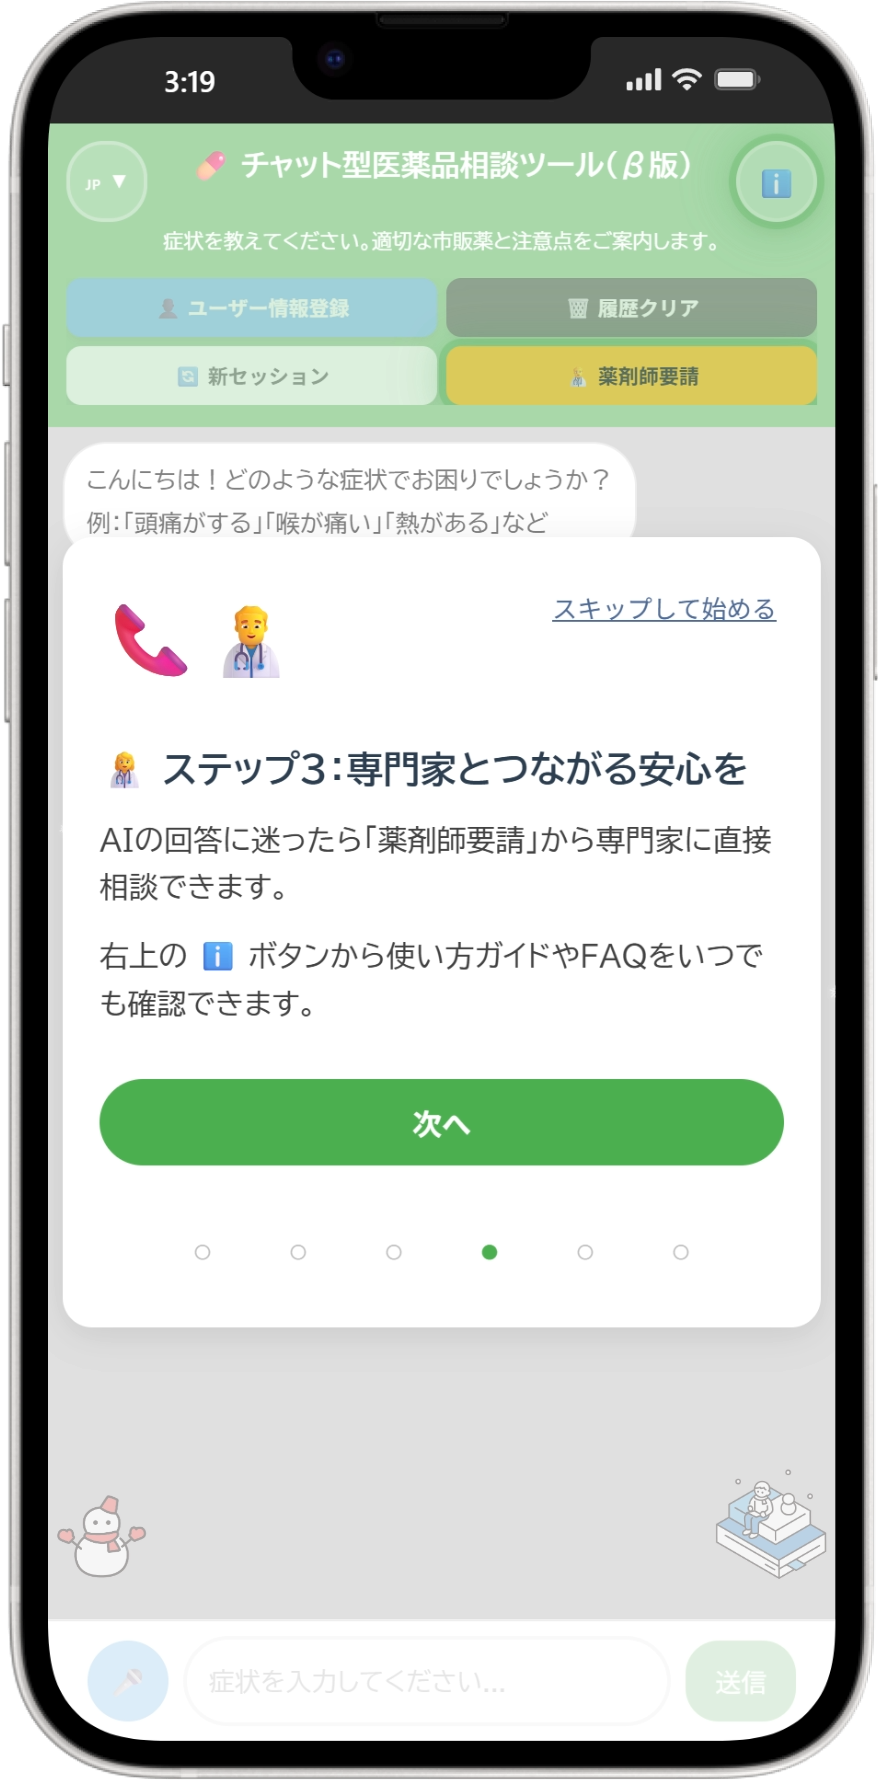
\includegraphics[width=\textwidth,keepaspectratio]{image/onboarding4.png}
\end{subfigure}
\begin{subfigure}[t]{0.17\textwidth}
  \centering
  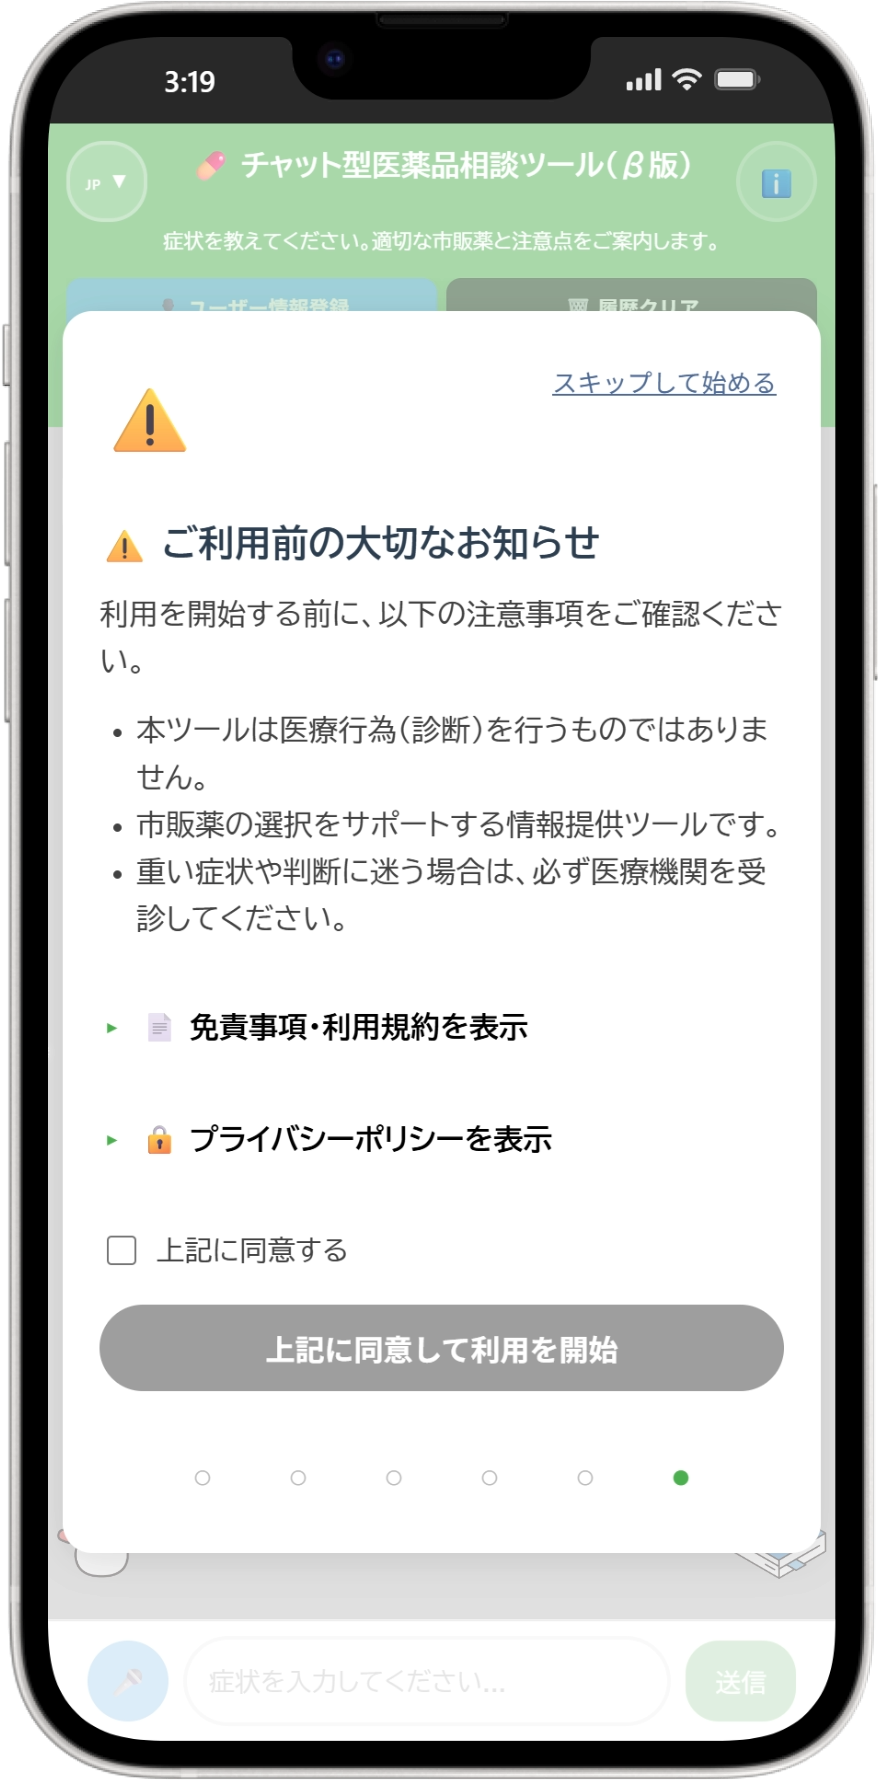
\includegraphics[width=\textwidth,keepaspectratio]{image/onboarding6.png}
\end{subfigure}
\end{center}
\caption{直感的なオンボーディングガイド（言語選択・利用注意・操作案内）\\
音声入力・読み上げ対応により、高齢者や文字入力が苦手な利用者にも配慮している。}
\label{fig:onboarding}
\end{figure}

\subsection*{期待される効果}
短期的には、本提案のシステムを通じて、ドラッグストアや自宅など身近な環境から、時間や場所の制約を受けずに医薬品の相談ができるようになる。市販薬選びに不安を抱える利用者に対して、具体的な製品候補と注意点を整理して提示でき、\textbf{相談の質の向上}に寄与する。さらに、図\ref{fig:carousel-all}に示すようにカルーセル型UIへ移行することで、推奨された医薬品をパッケージ画像・商品名・効能のカード形式でスワイプしながら確認できるようになる。文章を読み解く必要がなく、視覚的に候補を比較できるため、\textbf{推奨結果の認識しやすさと選択への安心感}が向上する。このUIはWebアプリ・LINEチャット・店頭タブレットのいずれにも展開し、プラットフォームを問わず直感的な医薬品選択を支援する。

中期的には、禁忌・アレルギーをルールで先に除外し、推奨根拠を説明可能な形で提示することにより、誤選択リスクを系統的に減らすことが期待される。既往症や併用薬を考慮した提案や、市販薬依存のリスクが高い成分を避けるブレーキ機能を、日常的な相談フローに組み込める点が重要である。

さらに、潜在空間ベクトル類似度を用いることで、多様な表現から共通する症状意味を捉え、推奨精度の向上が見込まれる。4言語対応と組み合わせることで、訪日外国人や多文化環境においても同等の支援を提供でき、\textbf{多言語での公平なアクセス}と店舗スタッフの言語負担軽減の効果もある。

長期的には、過疎地や離島などドラッグストアの少ない地域における「薬を相談して買う場所がない」という課題を和らげ、住む場所による健康格差の縮小に寄与することを目指す。専門家の知見をシステムとして共有し、「どこでも・誰にでも同じレベルの説明と提案が届く」状態を実現することで、セルフメディケーションを安心して行える土台を整える。

\subsection*{評価指標（どこまで測るか）}
以下の指標は現時点で想定している目標値（目安）であり、テストケース数・データセットの詳細は採択後にPMと相談して確定する。なお、応答時間については既に本番環境（GCP Cloud Run）で稼働中のシステムの実測値をもとに設定している。
\begin{table}[H]
\centering
\begin{tabularx}{\linewidth}{llX}
\toprule
種別 & 指標 & 目標・測定方法（目安） \\
\midrule
安全性 & 禁忌判定成功率 & 99\%以上。年齢・妊娠・既往症別のテストケースで検証 \\
安全性 & アレルギー成分検出率 & 100\%（成分単位の網羅的チェック） \\
安全性 & リスク入力ブロック率 & 100\%（プロンプトインジェクション・緊急ワード含む） \\
品質・性能 & 推奨一致率 & 薬剤師監修者が選んだ推奨との一致率（テストケース$n \geq 50$件を未踏期間中に構築）。ルールベース単体との比較でハイブリッドによる改善を確認 \\
品質・性能 & 応答時間 & GCP Cloud Run上での実測値30秒以内（OpenAI API呼び出し含む） \\
アクセシビリティ & エラー/再入力率 & 20\%以下（症状入力がリジェクトされ再入力が必要になったセッションの割合。セッションログから自動集計） \\
アクセシビリティ & 多言語完了率 & 85\%以上（英語・中国語・韓国語ユーザーが推奨結果まで到達した割合。言語別セッションログで計測） \\
\bottomrule
\end{tabularx}
\end{table}

% ========== ④ 具体的な進め方と予算 ==========
\section*{\ding{175} 具体的な進め方と予算}

\subsection*{(1) 主に開発を行う場所}
自宅（Windows 11、デスクトップ）および大学・外出先（MacBook Pro、ノートPC）。

\subsection*{(2) 使用する計算機環境（ハード・OS）}
\begin{itemize}[nosep,leftmargin=1em]
  \item \textbf{自宅}：Windows 11 Home、AMD Ryzen 9 9950X（16コア/32スレッド）、メモリ64GB、NVIDIA GeForce RTX 4070 SUPER
  \item \textbf{大学・外出先}：MacBook Pro（2020、Intel Core i7、メモリ16GB、macOS）
\end{itemize}

\subsection*{(3) 使用する言語・ツール}
\begin{table}[H]
\centering
\small
\begin{tabular}{@{}ll@{}}
\toprule
カテゴリ & ツール・言語 \\
\midrule
言語・フレームワーク & Python 3.11, Flask 3.x, Gunicorn \\
データベース & PostgreSQL（本番: Neon, 将来的に GCP Cloud SQL も併用検討）, SQLite（開発） \\
API & OpenAI API（GPT-4o-mini：NLU/応答生成, \textbf{text-embedding-3-small：潜在空間ベクトル生成}）, DeepL API（無料枠） \\
ライブラリ & pandas, numpy（コサイン類似度計算を含む）, pyahocorasick（症状辞書検索） \\
テスト・CI & pytest, GitHub Actions \\
インフラ & GCP Cloud Run、GCP Cloud SQL（PostgreSQL、検討中）、Neon（PostgreSQL） \\
\bottomrule
\end{tabular}
\end{table}

\subsection*{(4) 作業の分担}
個人開発のため、該当なし。

\subsection*{(5) 開発に使う手法}
既存リポジトリをベースとした継続開発。単体・統合・シナリオテストを拡充しつつ、Phase1→2→3 の順で段階的にマージし、各段階で評価可能な状態を維持する。禁忌ルールやフロー設計の妥当性については、薬剤師・登録販売者等の専門家に、8月後半〜12月末の間で2週間に1〜2回程度、一定の完成段階で監修・レビューを依頼する。Phase完了後（未踏期間内）にはよりしっかりとした監修を受け、安全性と現場感覚の両面から検証する予定である。

\subsection*{(6) 開発線表（いつまでに何をするか）}

\begin{figure}[H]
\centering

\includegraphics[width=\textwidth,keepaspectratio]{gantt_chart.png}
\caption{開発スケジュール（2026.06～2027.03）。Phase2で既存5層防御との結合を完了する。}
\end{figure}

\begin{table}[H]
\centering
\small
\begin{tabular}{@{}c@{\quad}l@{\quad}>{\raggedright\arraybackslash}p{\dimexpr\linewidth-15em\relax}@{}}
\toprule
時期 & 月 & 主な内容 \\
\midrule
開始 & 2026年6月（後半） & 環境・リポジトリ整理、既存テスト・CI確認、9ヶ月計画の詳細化、PM・IPAとのキックオフ \\
第1期 & 7月 & 潜在空間 Phase1: 埋め込みAPI利用設計、約8,000品目の医薬品の埋め込みベクトルをDBに事前計算・保存、コサイン類似度計算の単体テスト（n$\geq$50ケース）通過、ルールベースとの並行評価インターフェース動作確認まで完了。（※7月末は試験のため開発少なめ） \\
第2期 & 8月 & \textbf{【Phase1 完了】}上記deliverable達成を確認後、評価用データ・シナリオの整備。Phase2 設計（重み・動的重み付け） \\
専門家監修 & 8月後半～12月末 & 2週間に1〜2回程度、一定の完成段階で薬剤師・登録販売者等に監修・レビューを依頼。Phase完了後にしっかりとした監修を受ける。 \\
第3期 & 9月 & Phase2: ハイブリッドスコアリング関数の実装、既存5層防御との結合、統合テスト一式通過。\textbf{【Phase2 完了】}既存安全性指標（禁忌99\%・アレルギー98\%）を維持していることを確認。 \\
第4期 & 10月 & 安全性検証（禁忌・アレルギー検出率の維持）、パフォーマンス・レイテンシ確認、不具合修正 \\
第5期 & 11月 & Phase3: 薬剤師監修テストケース（n$\geq$50件）でルールベース単体との推奨一致率を比較し、ハイブリッドによる改善を数値で確認。パラメータ設定根拠を含む評価レポートを提出可能な状態に完成。\textbf{【Phase3 完了】} \\
第6期 & 12月 & ドキュメント整備（技術文書・README・API説明）、運用周り改善 \\
第7期 & 2027年1月 & 残タスク消化、デモ・動画の準備、成果報告書の下書き（※1月末は試験のため開発少なめ） \\
終了 & 2月～3月12日 & 成果報告書・実績報告書の取りまとめ、提出物の最終確認 \\
\bottomrule
\end{tabular}
\end{table}

\subsection*{(7) 開発にかかわる時間帯と時間数}
開発時間帯は、平日は放課後〜夜、土日祝は午前〜夕方を中心に確保する。開発期間は2026年6月22日～2027年3月12日（約9ヶ月、平日178日・土日祝86日）とする。通常期は平日3時間/日、土日祝は8時間/日とする。8月第2週から9月末までは夏休みを活用し、平日5時間/日、土日祝は8時間/日とする。7月末と1月末は学業の試験期のため、該当する4週は週15時間程度に抑える。以上を平日178日・土日祝86日の内訳に応じて按分し、\textbf{合計 1,295時間}を申請する（上限1,440時間以内）。内訳は下表のとおりである。

\begin{table}[H]
\centering
\small
\begin{tabular}{@{}llrr@{}}
\toprule
期間 & 内容 & 1日あたり時間 & 小計（時間） \\
\midrule
試験期（4週） & 7月末1週、1月末3週 & 週15時間 & 60 \\
夏休み期 & 8月第2週～9月末（平日・土日祝の日数に応じて按分） & 平日5h/日、土日祝8h/日 & 約302 \\
通常期 & 上記以外の日 & 平日3h/日、土日祝8h/日 & 約933 \\
\midrule
\multicolumn{3}{r}{合計} & 1,295 \\
\bottomrule
\end{tabular}
\end{table}

\subsection*{(8) 予算内訳}
申請金額は、1,295時間 × 2,100円/時間（税抜）＝ \textbf{2,719,500円}（税抜）とする。未踏では委託金は作業時間に基づいて支払われ、支出に条件はつかない。下表の必要経費はプロジェクト遂行に充てる目安であり、契約金額（作業時間ベース）とは無関係である。

\begin{table}[H]
\centering
\begin{tabularx}{\linewidth}{l>{\raggedright\arraybackslash}Xr}
\toprule
費目 & 内容 & 概算（円） \\
\midrule
OpenAI API & 埋め込み・LLM呼び出し（開発・検証・本番） & 40,000～60,000 \\
DeepL API & 多言語応答用（無料枠超過時・開発・検証） & 0～15,000 \\
GCP・Neon & Cloud Run・Cloud SQL（PostgreSQL）、Neon（PostgreSQL）利用料（開発・本番） & 5,000～25,000 \\
専門家監修 & 薬剤師・登録販売者等による内容監修・レビュー謝礼（8月後半～12月末で2週間に1～2回程度、Phase完了後にしっかりとした監修を受ける） & 50,000～120,000 \\
書籍・文献 & 機械学習・NLP・医薬品・セキュリティ関連 & 15,000～25,000 \\
ドメイン・その他 & ドメイン更新、開発用ツール等 & 5,000～10,000 \\
\bottomrule
\end{tabularx}
\end{table}

実際の支出は作業進捗に応じて行い、実績報告書で報告する。DeepL API は原則無料枠で利用し、超過分は上記予算から充てる。

% ========== ⑤ 提案者の腕前 ==========
\section*{\ding{176} 提案者（たち）の腕前を証明できるもの}

\begin{itemize}[nosep]
\item \textbf{本システム}: 医薬品推奨システムを個人で設計・開発し、公開運用中（\url{https://medicine.yutok.dev/}）。GitHubリポジトリ：\url{https://github.com/32Lwk/medicine-recommend-system}。本システムの設計・実装はすべて自分で行った。5層防御・ルールベーススコアリング・ハイブリッドNLU（辞書＋LLMフォールバック）を実装済み。4言語対応、GCP Cloud Run・Neon（PostgreSQL）本番運用の実績あり。未踏期間では、潜在空間の設計・実装と評価を新規に実施する。
\item \textbf{技術スタック}: Python（中級）、Flask、PostgreSQL、OpenAI API を実務レベルで使用している。登録販売者資格を2025年10月に取得しており、登録販売者として得た知見をルール設計・用語選定に活かしている。情報処理の知識をシステム設計に活かしている。
\item \textbf{受賞歴}：
\begin{itemize}[nosep,leftmargin=1em]
\item \makebox[9em][l]{2022年7月}（高校時代）：缶サット甲子園 和歌山大会 優勝
\item \makebox[9em][l]{2022年12月}（高校時代）：きのくにプログラミングコンテスト 最優秀賞
\item \makebox[9em][l]{2025年2月}：AWSデジタル社会実現ツアー2025 名古屋本戦 本戦出場
\item \makebox[9em][l]{2025年11月}：ユメカタリ 学生生成AIコンテスト 最優秀賞
\item \makebox[9em][l]{2025年12月}：椙山女学園大学第13回ビジネスコンペティション 優秀賞
\item \makebox[9em][l]{2025年12月}：第9回和歌山県データ利活用コンペティション クオリティソフト賞
\item \makebox[9em][l]{2026年1月}：doda アイデアコンペティション 審査員特別賞
\end{itemize}
\item \textbf{資格}: 基本情報技術者、登録販売者。
\item \textbf{デモ}: 環境依存を避けるため、\textbf{2～3分のデモ動画}を用意し、提出資料（Google Drive）に同梱する。二次審査時にも提示する。
\end{itemize}

% ========== ⑥ 特記事項 ==========
\section*{\ding{177} プロジェクト遂行にあたっての特記事項}

\begin{itemize}[nosep]
\item \textbf{学業との両立}: 名古屋大学理学部物理学科2年生（在学中）。指導教員はいない。学業との両立は自己管理で対応する。2年生のため研究室には未配属であり、在籍研究室は該当しない。名古屋大学の学則上、学外の委託事業への参加および報酬受領について制度上の問題がないことを確認済みである。
\item \textbf{組織・上司}: 該当なし（学生・個人開発）。マツモトキヨシでのアルバイトは継続するが、プロジェクト開発を優先する時間を確保する。繁忙期はアルバイトを減らし、夏休みは開発に集中する方針とする。アルバイト業務上で知り得た顧客情報・社内情報は一切本プロジェクトに利用しておらず、知的財産上の問題はない。
\item \textbf{進学・就職・転職・転居}: 開発期間中は特になし。
\item \textbf{チーム}: 個人開発のため、該当なし。
\item \textbf{未成年・保護者}: 該当なし（成年）。
\item \textbf{PM・IPAへの要望・固有の事情}: 特になし。提案書作成に generative AI を利用した（文章の推敲・構成検討の補助）。利用箇所は上記のとおりである。
\end{itemize}

% ========== ⑦ IT以外 ==========
\section*{\ding{178} IT以外の勉強、特技、生活、趣味など}

\textbf{勉強}: 専攻は物理学・宇宙物理学である。松原隆彦著「宇宙のかたち」を読み、夜空に一様に広がって見える星々にも実は奥行きがあること、そして宇宙には銀河フィラメントのように銀河が連なる構造や、逆に銀河がほとんど存在しないボイドといった、目には見えない大規模な構造が広がっていることを知った。そのスケールの大きさと構造の神秘に強く惹かれ、宇宙物理学を志した。大学進学時には情報系の学科も候補にあったが、まずは自然現象を支える数理やモデル化の力を軸に宇宙を理解したいと考え、理学部物理学科を選んだ。物理学を通じて培ったデータやモデルを扱う姿勢は、本プロジェクトにおける医薬品データの設計やルール策定にも活きている。将来的には、観測データ解析や機械学習を用いた宇宙構造の研究にも取り組みたいと考えており、その過程で深める数理的思考やデータ解析の視点を、社会課題への応用にも活かしていきたい。

\textbf{特技・スポーツ}: 中学で軟式テニス部、高校で硬式テニス部に所属。中学・高校を通じてテニスを続けてきた経験から、小さな改善の積み重ねが大きな変化を生むことを体感している。フォームを少し変えるだけで球筋が変わる、その繰り返しが成長につながるという感覚は、本システムの段階的なフェーズ開発（Phase1$\to$2$\to$3）にも反映されている。現在はランニングも日課の一つであり、勉強や開発で頭がいっぱいになったときに走ることで気持ちをリセットしている。ランニング中にプロジェクトのアイデアや実装方針が整理されることも多く、開発と生活をつなぐ大切な時間になっている。

\textbf{生活で大切にしていること}: 相手の立場に立って考え、安心感を与える行動。登録販売者として、専門知識を一方的に伝えるのではなく、相手の困りごとを汲み取り、理解できる言葉で説明することを意識している。

\textbf{趣味}: 散歩、一人で考え事をする時間、ランニング。

% ========== ⑧ 将来のIT ==========
\section*{\ding{179} 将来のITについて思うこと・期すること}

宇宙物理学では、目に見えない暗黒物質が銀河の大規模構造を支えているように、社会においても「見えない構造」が人の判断を静かに支えている。潜在空間は、言葉の意味という見えない構造をデータの中に見出す試みであり、そこに星間ガスの分布や銀河フィラメントを観測する知的興奮と同じものを感じる。ITがこれからの社会インフラになるとき、ブラックボックスのまま見えない構造に丸投げするのではなく、構造を理解し説明できる形で社会に接続することが、物理学者の視点からも不可欠だと考えている。

医療・金融・交通・行政など、設計が安全や人生に直結する領域では、スピード・新規性に加え、誤らないこと・説明可能性・止まらないことがより求められる。生成AIで実装のハードルは下がったが、「どこを機械に任せ、どこを人が責任を持つか」という設計判断の重要性は増している。本提案で目指している、誤りを防ぎ説明可能なシステムづくりは、その一歩だと考えている。

未踏修了後は、まず大規模・高信頼性が求められるシステムに携われる環境でエンジニアとして経験を積みたい。社会インフラや基盤技術に近い領域で、設計から運用まで責任を持つ経験を通じて技術を鍛えたい。そのうえで、観測データ解析や機械学習を用いた宇宙構造の研究と社会課題解決の両輪でアプローチするプロジェクトの立ち上げや、未踏アドバンストへの挑戦も視野に入れている。未踏が「実装できる思想家」を育てる場であり続けてほしいと期待している。

\end{document}
